% Options for packages loaded elsewhere
\PassOptionsToPackage{unicode}{hyperref}
\PassOptionsToPackage{hyphens}{url}
%
\documentclass[
  ,man,mask,floatsintext]{apa6}
\usepackage{amsmath,amssymb}
\usepackage{lmodern}
\usepackage{iftex}
\ifPDFTeX
  \usepackage[T1]{fontenc}
  \usepackage[utf8]{inputenc}
  \usepackage{textcomp} % provide euro and other symbols
\else % if luatex or xetex
  \usepackage{unicode-math}
  \defaultfontfeatures{Scale=MatchLowercase}
  \defaultfontfeatures[\rmfamily]{Ligatures=TeX,Scale=1}
\fi
% Use upquote if available, for straight quotes in verbatim environments
\IfFileExists{upquote.sty}{\usepackage{upquote}}{}
\IfFileExists{microtype.sty}{% use microtype if available
  \usepackage[]{microtype}
  \UseMicrotypeSet[protrusion]{basicmath} % disable protrusion for tt fonts
}{}
\makeatletter
\@ifundefined{KOMAClassName}{% if non-KOMA class
  \IfFileExists{parskip.sty}{%
    \usepackage{parskip}
  }{% else
    \setlength{\parindent}{0pt}
    \setlength{\parskip}{6pt plus 2pt minus 1pt}}
}{% if KOMA class
  \KOMAoptions{parskip=half}}
\makeatother
\usepackage{xcolor}
\usepackage{longtable,booktabs,array}
\usepackage{calc} % for calculating minipage widths
% Correct order of tables after \paragraph or \subparagraph
\usepackage{etoolbox}
\makeatletter
\patchcmd\longtable{\par}{\if@noskipsec\mbox{}\fi\par}{}{}
\makeatother
% Allow footnotes in longtable head/foot
\IfFileExists{footnotehyper.sty}{\usepackage{footnotehyper}}{\usepackage{footnote}}
\makesavenoteenv{longtable}
\usepackage{graphicx}
\makeatletter
\def\maxwidth{\ifdim\Gin@nat@width>\linewidth\linewidth\else\Gin@nat@width\fi}
\def\maxheight{\ifdim\Gin@nat@height>\textheight\textheight\else\Gin@nat@height\fi}
\makeatother
% Scale images if necessary, so that they will not overflow the page
% margins by default, and it is still possible to overwrite the defaults
% using explicit options in \includegraphics[width, height, ...]{}
\setkeys{Gin}{width=\maxwidth,height=\maxheight,keepaspectratio}
% Set default figure placement to htbp
\makeatletter
\def\fps@figure{htbp}
\makeatother
\setlength{\emergencystretch}{3em} % prevent overfull lines
\providecommand{\tightlist}{%
  \setlength{\itemsep}{0pt}\setlength{\parskip}{0pt}}
\setcounter{secnumdepth}{-\maxdimen} % remove section numbering
% Make \paragraph and \subparagraph free-standing
\ifx\paragraph\undefined\else
  \let\oldparagraph\paragraph
  \renewcommand{\paragraph}[1]{\oldparagraph{#1}\mbox{}}
\fi
\ifx\subparagraph\undefined\else
  \let\oldsubparagraph\subparagraph
  \renewcommand{\subparagraph}[1]{\oldsubparagraph{#1}\mbox{}}
\fi
\newlength{\cslhangindent}
\setlength{\cslhangindent}{1.5em}
\newlength{\csllabelwidth}
\setlength{\csllabelwidth}{3em}
\newlength{\cslentryspacingunit} % times entry-spacing
\setlength{\cslentryspacingunit}{\parskip}
\newenvironment{CSLReferences}[2] % #1 hanging-ident, #2 entry spacing
 {% don't indent paragraphs
  \setlength{\parindent}{0pt}
  % turn on hanging indent if param 1 is 1
  \ifodd #1
  \let\oldpar\par
  \def\par{\hangindent=\cslhangindent\oldpar}
  \fi
  % set entry spacing
  \setlength{\parskip}{#2\cslentryspacingunit}
 }%
 {}
\usepackage{calc}
\newcommand{\CSLBlock}[1]{#1\hfill\break}
\newcommand{\CSLLeftMargin}[1]{\parbox[t]{\csllabelwidth}{#1}}
\newcommand{\CSLRightInline}[1]{\parbox[t]{\linewidth - \csllabelwidth}{#1}\break}
\newcommand{\CSLIndent}[1]{\hspace{\cslhangindent}#1}
\ifLuaTeX
\usepackage[bidi=basic]{babel}
\else
\usepackage[bidi=default]{babel}
\fi
\babelprovide[main,import]{british}
% get rid of language-specific shorthands (see #6817):
\let\LanguageShortHands\languageshorthands
\def\languageshorthands#1{}
% Manuscript styling
\usepackage{upgreek}
\captionsetup{font=singlespacing,justification=justified}

% Table formatting
\usepackage{longtable}
\usepackage{lscape}
% \usepackage[counterclockwise]{rotating}   % Landscape page setup for large tables
\usepackage{multirow}		% Table styling
\usepackage{tabularx}		% Control Column width
\usepackage[flushleft]{threeparttable}	% Allows for three part tables with a specified notes section
\usepackage{threeparttablex}            % Lets threeparttable work with longtable

% Create new environments so endfloat can handle them
% \newenvironment{ltable}
%   {\begin{landscape}\centering\begin{threeparttable}}
%   {\end{threeparttable}\end{landscape}}
\newenvironment{lltable}{\begin{landscape}\centering\begin{ThreePartTable}}{\end{ThreePartTable}\end{landscape}}

% Enables adjusting longtable caption width to table width
% Solution found at http://golatex.de/longtable-mit-caption-so-breit-wie-die-tabelle-t15767.html
\makeatletter
\newcommand\LastLTentrywidth{1em}
\newlength\longtablewidth
\setlength{\longtablewidth}{1in}
\newcommand{\getlongtablewidth}{\begingroup \ifcsname LT@\roman{LT@tables}\endcsname \global\longtablewidth=0pt \renewcommand{\LT@entry}[2]{\global\advance\longtablewidth by ##2\relax\gdef\LastLTentrywidth{##2}}\@nameuse{LT@\roman{LT@tables}} \fi \endgroup}

% \setlength{\parindent}{0.5in}
% \setlength{\parskip}{0pt plus 0pt minus 0pt}

% Overwrite redefinition of paragraph and subparagraph by the default LaTeX template
% See https://github.com/crsh/papaja/issues/292
\makeatletter
\renewcommand{\paragraph}{\@startsection{paragraph}{4}{\parindent}%
  {0\baselineskip \@plus 0.2ex \@minus 0.2ex}%
  {-1em}%
  {\normalfont\normalsize\bfseries\itshape\typesectitle}}

\renewcommand{\subparagraph}[1]{\@startsection{subparagraph}{5}{1em}%
  {0\baselineskip \@plus 0.2ex \@minus 0.2ex}%
  {-\z@\relax}%
  {\normalfont\normalsize\itshape\hspace{\parindent}{#1}\textit{\addperi}}{\relax}}
\makeatother

% \usepackage{etoolbox}
\makeatletter
\patchcmd{\HyOrg@maketitle}
  {\section{\normalfont\normalsize\abstractname}}
  {\section*{\normalfont\normalsize\abstractname}}
  {}{\typeout{Failed to patch abstract.}}
\patchcmd{\HyOrg@maketitle}
  {\section{\protect\normalfont{\@title}}}
  {\section*{\protect\normalfont{\@title}}}
  {}{\typeout{Failed to patch title.}}
\makeatother

\usepackage{xpatch}
\makeatletter
\xapptocmd\appendix
  {\xapptocmd\section
    {\addcontentsline{toc}{section}{\appendixname\ifoneappendix\else~\theappendix\fi\\: #1}}
    {}{\InnerPatchFailed}%
  }
{}{\PatchFailed}
\usepackage{lineno}

\linenumbers
\usepackage{csquotes}
\usepackage{float}
\usepackage{framed}
\usepackage{caption}
\usepackage{setspace}
\usepackage{amsmath}
\usepackage{wrapfig}
\captionsetup[figure]{font={stretch=1, small}, skip=10pt}
\captionsetup[textbox]{name=Box,labelsep=period,labelfont=it}
\newfloat{textbox}{thp}{lop}
\floatname{textbox}{Box}
\usepackage[most]{tcolorbox}
\definecolor{electricviolet}{rgb}{0.56, 0.0, 1.0}
\ifLuaTeX
  \usepackage{selnolig}  % disable illegal ligatures
\fi
\IfFileExists{bookmark.sty}{\usepackage{bookmark}}{\usepackage{hyperref}}
\IfFileExists{xurl.sty}{\usepackage{xurl}}{} % add URL line breaks if available
\urlstyle{same} % disable monospaced font for URLs
\hypersetup{
  pdftitle={Incentives for Registered Reports from a risk sensitivity perspective},
  pdflang={en-UK},
  hidelinks,
  pdfcreator={LaTeX via pandoc}}

\title{Incentives for Registered Reports from a risk sensitivity perspective}
\author{Anne M. Scheel\textsuperscript{1}, Leo Tiokhin\textsuperscript{1}, \& Daniël Lakens\textsuperscript{1}}
\date{}


\shorttitle{Risk-sensitive publication strategies}

\authornote{

Correspondence concerning this article should be addressed to Anne M. Scheel, Den Dolech 1, Atlas 9.417, 5600 MB, Eindhoven, The Netherlands. E-mail: \href{mailto:a.m.scheel@tue.nl}{\nolinkurl{a.m.scheel@tue.nl}}

}

\affiliation{\vspace{0.5cm}\textsuperscript{1} Eindhoven University of Technology}

\note{test}

\begin{document}
\maketitle

Registered Reports are an article format designed to reduce publication bias and `questionable research practices' (QRPs), which distort the published record of research findings in many scientific disciplines (Chambers, 2013; de Vries et al., 2018; Dickersin \& Min, 1993; Driessen, Hollon, Bockting, Cuijpers, \& Turner, 2015; Franco, Malhotra, \& Simonovits, 2014; Franco, Malhotra, \& Simonovits, 2016; Fraser, Parker, Nakagawa, Barnett, \& Fidler, 2018; Gerber, Green, \& Nickerson, 2001; Gopalakrishna et al., 2022; John, Loewenstein, \& Prelec, 2012; Kepes, Keener, McDaniel, \& Hartman, 2022; Makel, Hodges, Cook, \& Plucker, 2021; O'Boyle, Banks, \& Gonzalez-Mulé, 2017; Simmons, Nelson, \& Simonsohn, 2011; Stefan \& Schönbrodt, 2023).
In this format, peer review takes place before data collection and the decision to publish is made before authors, reviewers, and editors know the study results.
In addition to preventing editors from selectively rejecting unfavourable results (in particular negative or null results), this is thought to remove incentives for authors to hide, embellish, or misrepresent results because publication no longer depends on them
(Chambers, Dienes, McIntosh, Rotshtein, \& Willmes, 2015).
Initial evidence from psychology and neighbouring disciplines shows that Registered Reports indeed contain much higher rates of negative results than the standard literature (Allen \& Mehler, 2019; O'Mahony, 2023; Scheel, Schijen, \& Lakens, 2021).

Advocates of the format have argued that the pre-data publication guarantee should make Registered Reports particularly attractive to researchers (e.g., Chambers \& Tzavella, 2022).
The argument is that Registered Reports reduce uncertainty about whether and where a study will be published before authors have invested in conducting the study, and that such risk reduction is appealing
in a research climate that involves substantial publication pressure in many countries and disciplines (Gopalakrishna et al., 2022; Miller, Taylor, \& Bedeian, 2011; Paruzel-Czachura, Baran, \& Spendel, 2021; Tijdink, Vergouwen, \& Smulders, 2013; van Dalen, 2021; van Dalen \& Henkens, 2012; Waaijer, Teelken, Wouters, \& van der Weijden, 2018).
However, if strategic concerns about publishability indeed influence researchers' choices for or against Registered Reports, it is unlikely that they would always cause risk aversion (i.e., favouring Registered Reports as a low-risk option).
Researchers' willingness to take risks regarding publication success may instead vary depending on factors such as available resources, time pressure, or competition.
This could create situations in which Registered Reports remain unpopular and would never gain traction without additional incentives or interventions.
And indeed, although uptake is growing exponentially (Chambers \& Tzavella, 2022), the market share of Registered Reports is currently still much smaller than one might expect if authors saw them as unreservedly beneficial for their careers.
Here, we examine these possibilities with an agent-based simulation, modelling authors' choices between publication formats as decision making under risk to identify circumstances in which Registered Reports might be used highly selectively, or not at all.

\hypertarget{design-and-intended-functions-of-registered-reports}{%
\subsection{Design and intended functions of Registered Reports}\label{design-and-intended-functions-of-registered-reports}}

The review process of Registered Reports is split into two stages.
At Stage 1, reviewers evaluate a pre-study protocol containing the research questions, hypotheses, methods, and planned analyses of a proposed study.
In case of a positive decision, the journal issues an `in-principle acceptance' and commits to publishing the eventual report, regardless of the direction of the results.
Only after in-principle acceptance has been issued do authors move on to data collection and analysis and eventually complete the manuscript.
At Stage 2, the final report (now including the results) is subjected to a second round of peer review, but this time only to ensure that the study was carried out as planned, that the data pass any pre-specified quality checks, and that authors' conclusions are justified by the evidence.
Manuscripts can still be rejected at Stage 2, but only for substantial violations of the Stage-1 protocol or data that are uninterpretable or uninformative (e.g., caused by equipment failure), not for the direction or statistical significance of the results.

Through this process, Registered Reports address publication bias as well as so-called `questionable research practices' (QRPs).
These two problems are considered important contributors to psychology's replication crisis (Ferguson \& Heene, 2012; Wagenmakers, Wetzels, Borsboom, van der Maas, \& Kievit, 2012) and to research waste in the biomedical sciences (Chalmers \& Glasziou, 2009) because they skew the available evidence for scientific claims, causing overconfidence and inflated rates of false-positive inferences.
Publication bias can result from editors and reviewers disproportionately rejecting submissions with negative results (`reviewer bias,' Atkinson, Furlong, \& Wampold, 1982; Greenwald, 1975; Mahoney, 1977) or from researchers failing to submit negative results for publication (`file-drawering,' Ensinck \& Lakens, 2023; Franco et al., 2014; Rosenthal, 1979).
In Registered Reports, the
in-principle acceptance issued at Stage 1 addresses both of these issues:
Editors and reviewers cannot reject the Stage-2 report based on the direction of the results, which also reduces the incentives for authors to file-drawer the study in case of negative results.
QRPs are practices that exploit undisclosed flexibility in data collection and analysis, for example when analysing different justifiable combinations of variables, subsamples, and decision criteria, and only reporting the ones with favourable results, or by presenting \emph{post hoc} inferences as having been predicted \emph{a priori} (Agnoli, Wicherts, Veldkamp, Albiero, \& Cubelli, 2017; Fiedler \& Schwarz, 2016; Fraser et al., 2018; Gopalakrishna et al., 2022; John et al., 2012; Kerr, 1998; Simmons et al., 2011).
Registered Reports minimise the risk of QRPs via the two-stage review process, in which the Stage-1 protocol acts as a preregistration and reviewers' task during Stage-2 review is to flag any undisclosed deviations from it.

\hypertarget{efficacy-of-registered-reports}{%
\subsection{Efficacy of Registered Reports}\label{efficacy-of-registered-reports}}

Registered Reports were first launched in 2013 at the journal \emph{Cortex} (Chambers, 2013) and are now offered by over 300 journals, predominantly in the behavioural sciences and life sciences (see \url{cos.io/rr}).
Nearly 600 Registered Reports had been published by 2021, with uptake growing exponentially (Chambers \& Tzavella, 2022).
In Chapter 2, we analysed the first cohort of published Registered Reports in psychology and showed that the first hypothesis reported in these articles was supported in only \(44\%\) of cases, compared to \(96\%\) in a random sample of standard reports (Scheel et al., 2021).
Similarly low proportions of positive results were found in partially overlapping samples of Registered Reports in psychology and neuroscience (\(39.5\%\), Allen \& Mehler, 2019) and in psychology, neuroscience, health, and education (\(50.1\%\), O'Mahony, 2023).
These findings suggest that Registered Reports indeed reduce biases that inflate the rate of positive results in the standard literature.
However, the existing estimates are based on purely observational evidence and may thus be confounded by other systematic differences between Registered Reports and standard reports.

Systematic differences would act as confounders if they affected either the probability of a positive result when testing a true hypothesis (statistical power) or the base rate of true hypotheses.
The first option is not supported by current evidence:
A study comparing Registered Reports with matched controls found that Registered Reports have higher median sample sizes and, in blind reviews, are judged to be more rigorous in methodology and analysis and of higher overall quality (Soderberg et al., 2021).
Based on this finding, the increased amount of negative results in Registered Reports is unlikely to be an artifact of lower statistical power or poorer methods.
But the second option\(\,\)---\(\,\)a difference in the rate of true hypotheses, or the (prior) probability that the tested hypothesis is true\(\,\)---\(\,\)has not yet been directly studied.
The idea that Registered Reports might contain fewer true hypotheses has some plausibility:
If researchers expect that negative results are difficult to publish in standard reports but pose no problem in Registered Reports, they might selectively choose the Registered Report route when studying hypotheses that they think
will yield negative results.
If researchers additionally perceive the standard publication route as less costly (e.g., more habitual, more flexible, faster, requiring lower sample sizes, etc.), standard reports would plausibly remain the preferred option for hypotheses that researchers are more certain are true and will yield publishable results.

Such an effect could explain why both we and Allen \& Mehler (2019) found that replication studies in the Registered Reports literature had descriptively lower rates of positive results than original studies, although the difference was not significant in either case (\(39\%\) vs \(50\%\) in Scheel et al., 2021, and \(34\%\) vs \(45.5\%\) in Allen \& Mehler, 2019, though note that the studied samples partially overlap).
As we discussed in Chapter 2, replication attempts may more often than novel research be driven by the suspicion that the tested hypothesis is not true (and that the result of the original study was a false positive).
It might also partially explain differences between our results and those of O'Mahony (2023), who compared Registered Reports to standard reports that were matched on based on the publishing journal, time of publication, and to a lesser extent research topic, design, and studied population.
O'Mahony finds a difference in the positive result rate of Registered Reports and standard reports half as large as the one in our study (26 vs 52 percentage points), which compared Registered Reports with a random sample of standard reports (matched only on discipline).
Matching articles more closely could lead to more comparable prior probabilities of the hypotheses tested in both formats and thus account for part of this discrepancy.
However, the two studies also differ in the target population and estimand (O'Mahony analysed all tested hypotheses whereas Scheel et al.~focused on the first hypothesis per article), which makes the estimates difficult to compare.

Although differences between hypotheses tested in Registered Reports and standard reports remain speculative at this point, this consideration highlights the importance of understanding the costs and benefits of Registered Reports from the authors' perspective.
If current incentives cause Registered Reports to be used selectively in specific situations or for specific research questions, meta-scientists studying this emerging literature would need to take such factors into account.
Selective use could also lead to a situation in which Registered Reports become associated with certain types of results (e.g., negative results) and devalued if these results are deemed less interesting or important by the research community, making the format unattractive in the long run.
More generally, a better understanding of the incentives driving researchers' publication choices can help determine where, when, and by whom Registered Reports are likely to be used or avoided.
Such knowledge could then be used to identify areas in which Registered Reports may not gain popularity naturally and anticipate the need for further intervention (e.g., via policy) when there is a demand for unbiased results.

\hypertarget{author-incentives-for-registered-reports}{%
\subsection{Author incentives for Registered Reports}\label{author-incentives-for-registered-reports}}

Registered Reports are generally thought to `{[}neutralise{]} bad incentives' (Chambers, 2013, p. 609), in particular the incentive to exaggerate or misrepresent a study's results in order to make them more publishable in the standard literature.
This assumption is conditioned on the format:
Once authors have decided to take the Registered Report route, they can improve their publication chances only via the proposed research question and methods in Stage-1 review, and editors have an interest in selecting informative study designs because they are bound to publishing the study's results even when they turn out negative.
In contrast to standard reports, the results are thus no longer a main target to `hack' or select on, which should make them less biased and more trustworthy.

The incentives for choosing the Registered Reports route in the first place, however, are less clear.
Advocates of the format have argued that it `serve{[}s{]} the interests of individual scientists' (p.~12, Chambers \& Tzavella, 2022) because it reduces scientists' risk of investing in research projects whose results turn out to be difficult to publish.
The argument is based on the assumptions that researchers a) are under pressure to amass journal publications (which still are a central currency for hiring and promotion decisions, R. Müller, 2014; van Dalen \& Henkens, 2012) and b) face shortfalls in publication output when their studies yield negative results (which are more difficult to publish in the standard literature due to publication bias).
The following quote from a talk by Chris Chambers (\href{https://youtu.be/FiVI3cwVMZI?list=PLChfyH8TVDGmYENpXUDPaeeq2SLh8q9dt\&t=1047}{September 2021}) summarises this sentiment:

\begin{quote}
And the second main benefit, the one that really is the main big one, the big draw, is that as a researcher you can get your paper accepted before you even start your research and regardless of how the results turn out in the end. So no more playing the \emph{p}-value lottery, gambling on certain results going a certain way, otherwise you won't have your PhD or you won't get your next fellowship or your next grant\(\,\)---\(\,\)takes all of that pointless, and I think quite foolish, gambling out of the equation (\ldots)\footnote{\url{https://youtu.be/FiVI3cwVMZI?list=PLChfyH8TVDGmYENpXUDPaeeq2SLh8q9dt\&t=1047}, from minute 17:27}
\end{quote}

But would researchers ever prefer to gamble?
Typically, authors care not only about their studies being published at all, but also about the reputation of the publishing journal as well as citation rates (which are causally influenced by journal rank, Traag, 2021).
In standard reports, the career-relevant payoffs associated with a publication can thus vary from very low, for example when authors file-drawer a manuscript because the chances of success do not justify the cost of repeated submissions and revisions (Ensinck \& Lakens, 2023),
to very high, for example when a manuscript is published in an extremely high-impact journal like \emph{Nature} or \emph{Science} and frequently cited.
Compared to this, the payoffs from Registered Reports have lower variance:
Registered Reports minimise not only the chances of a very low payoff (no publication at all), but also those of a very high payoff (a highly-cited publication in a top journal, unless the Registered Report is conducted at a top journal).
Therefore, as long as the payoff associated with a published Registered Report is not always on par with the best possible outcome of the standard publication route,
there will be situations in which the standard route\(\,\)---\(\,\)`taking the gamble'\(\,\)---\(\,\)is more beneficial for researchers.

\hypertarget{publication-strategies-as-decision-making-under-risk}{%
\subsection{Publication strategies as decision making under risk}\label{publication-strategies-as-decision-making-under-risk}}

Which are those situations?
Because the payoffs of Registered Reports and the standard publication route differ in variance, authors' choice between the two formats represents \emph{decision making under risk}.
This framing allows us to use tools from the literature on risk-sensitive behaviour to study when Registered Reports serve the interests of individual scientists less well than standard reports.
Here, we use risk-sensitivity theory to model factors that influence risk preferences and simulate their effects on researchers' publication strategies.
Following Winterhalder, Lu, \& Tucker (1999), we define \emph{risk} as `unpredictable variation in the outcome of a behavior, with consequences for an organism's fitness or utility' (p.~302).
\emph{Risk aversion} thus means preferring a low-variance option over a high-variance option, and \emph{risk proneness} the reverse.\footnote{Note that these definitions differ from those used in expected utility theory, where risk aversion, risk proneness, and risk indifference are defined as concave-down, convex-up, and linear utility functions, respectively.}
Organisms are \emph{risk sensitive} when they are not only sensitive to the average of outcomes of different behavioural options but also to their variance.

Risk-sensitivity theory is a normative theory developed in behavioural ecology to explain the foraging behaviour of animals.
It was originally designed to determine the optimal food-acquisition strategy for an animal faced with a choice between a relatively stable (low-variance) food source and a risky (high-variance) source that sometimes yields large payoffs and sometimes small payoffs (or none at all).
Organisms are predicted to be sensitive to such differences in risk when payoffs (e.g., the amount of food) have non-linear consequences for the organism's survival or reproductive fitness.
This is the case when, for example, additional increments of food yield smaller and smaller returns for an animal's fitness, or when amounts below a certain threshold would cause starvation.
In psychology and economics, analogous problems in human decision-making are usually studied with utility-based theories, most prominently expected utility theory and prospect theory.
The predictions of all three theories overlap substantially, but risk-sensitivity theory uses fitness instead of utility as its central currency.
This overcomes weaknesses of expected utility theory and prospect theory caused by the conceptual vagueness of utility (e.g., `utility is whatever is maximised by human choices,' Cubitt, Starmer, \& Sugden, 2001).
Despite its initially narrow scope, risk-sensitivity theory has proven itself as a powerful framework for explaining risk-sensitive behaviour in a wide range of situations and species, including humans (Kacelnik \& Bateson, 1996; Mishra, 2014; Winterhalder et al., 1999).

\hypertarget{the-present-study}{%
\subsection{The present study}\label{the-present-study}}

In the following, we apply
risk-sensitivity theory to
the situation of researchers faced with the choice of conducting a Registered Report or pursuing the standard publication route.
Using a simulation model, we explore how four aspects of academic careers and incentive structures that are relevant to risk sensitivity may affect researchers' publication strategies:
whether additional publications yield decreasing or increasing returns for career success, empirical pace (the frequency at which studies can be completed), publication targets that must be met to continue or further one's career, and competition.
Our goal is to understand in which circumstances Registered Reports should be particularly attractive, particularly unattractive, or particularly prone to selective use.
The results of this analysis may help anticipate research fields and career stages in which the format is unlikely to take foot without additional changes to norms, incentives, or policy, and flag situations in which the results of published Registered Reports may be particularly difficult to compare to the normal literature.
The following sections outline central concepts of risk-sensitivity theory, relate them to characteristics of academic careers, and describe an evolutionary simulation model in which their effects on researchers' risk-sensitive publication decisions are examined.

\hypertarget{conceptual-application-of-risk-sensitivity-theory-to-publication-decisions}{%
\section{Conceptual application of risk-sensitivity theory to publication decisions}\label{conceptual-application-of-risk-sensitivity-theory-to-publication-decisions}}

This section describes general factors that affect the role of risk for individual's fitness and connects these factors to relevant elements of academic careers.
In this context, risk-sensitivity theory's focus on reproductive fitness as the central outcome may be seen as misguided.
But although researchers do not forage, grow, reproduce, and die in the \emph{biological} sense (except in their role as human beings in general, of course), they undoubtedly are concerned with factors that influence 1) their survival and 2) the propagation of their traits in an \emph{academic} sense.
Even if we were to assume that researchers are not consciously trying to maximise their `academic fitness', a competitive job market will by definition select for individuals whose past behaviour increased their prospects.
Such competition can create bottlenecks between early-career and tenured positions in many academic disciplines, which inevitably induce a selection pressure for career-promoting behaviours Higginson \& Munafò (2016).

In applying risk-sensitivity theory to researchers' publishing behaviour, we will therefore conceptualise fitness as career success.
This decision does not imply that career success is the only or the proximal motivation for researchers' behaviour in practice, just as evolutionary theory does not imply that reproductive success is the only or the proximal motivation for human behaviour in everyday life.
However, we do assume that selection for career-promoting behaviours has a noticeable impact on research practice.



\par\vspace{.8\baselineskip}
\begin{figure}

{\centering 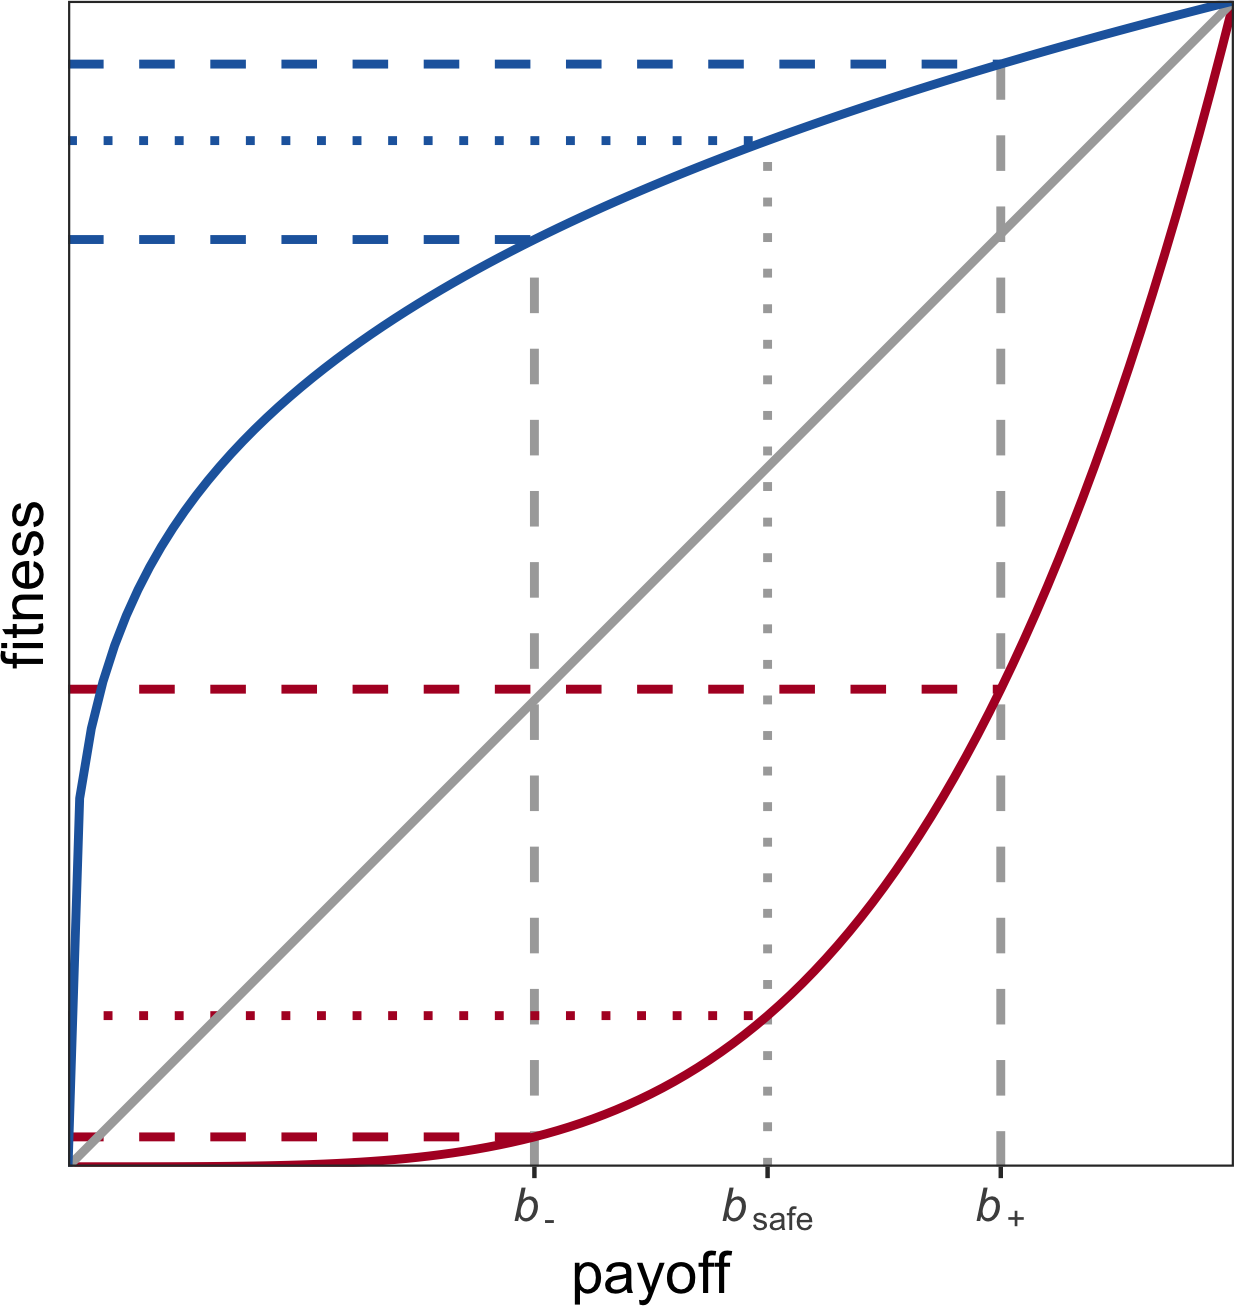
\includegraphics[width=0.5\linewidth]{rr-risk-sensitivity_files/figure-latex/fitnessplot-1} 

}

\caption{Consequences of non-linear fitness functions. Payoffs \(b_-\), \(b_{safe}\), and \(b_+\) are converted into fitness with a diminishing (blue), linear (grey), or increasing (red) returns function.}\label{fig:fitnessplot}
\end{figure}
\par\vspace{.5\baselineskip}

\hypertarget{non-linear-fitness-functions}{%
\paragraph{Non-linear fitness functions}\label{non-linear-fitness-functions}}

The first and perhaps most ubiquitous factor leading individuals to be risk sensitive are non-linear relationships between the outcomes of an individual's behaviour (e.g., harvested food items, publications) and its reproductive success (Kacelnik \& Bateson, 1997).
Consider two options, \(O_{safe}\) and \(O_{risky}\).
\(O_{safe}\) always gives the same payoff \(b_{safe}\), whereas \(O_{risky}\) gives either a low payoff \(b_-\) or a high payoff \(b_+\), each with probability \(\frac{1}{2}\).
When \(b_{safe} = \frac{(b_- + b_+)}{2}\), \(O_{safe}\) and \(O_{risky}\) have the same expected payoff.
However, we would only expect an individual to be indifferent between the two options if the consequences of their payoffs for the individual's fitness are linear.
When the function relating payoffs to fitness is instead convex or concave (yielding increasing or diminishing returns, respectively), the expected fitness of \(O_{safe}\) and \(O_{risky}\) will differ and shift the individual's preference towards risk proneness or risk aversion.
An illustration of this example is shown in Figure~\ref{fig:fitnessplot}:
While the payoffs \(b_-\), \(b_{safe}\), and \(b_+\) are equidistant on the x-axis, \(b_{safe}\) is associated with greater fitness than the average of \(b_-\) and \(b_+\) when the function is concave, and with lower fitness when the function is convex.
In other words, \(O_{safe}\) has greater expected fitness than \(O_{risky}\) when returns are diminishing, and \(O_{risky}\) has greater expected fitness than \(O_{safe}\) when returns are increasing.

Non-linear relationships are arguably the norm in the natural world and linear relationships the exception.
This plausibly holds for academia as well, where the effect of publication success on researchers' career success might change over time:
For early-career researchers, small increases in the number or impact of publications may have an accelerated effect on career success, whereas established professors may care little about any one additional publication to their record.

\hypertarget{number-of-decision-events-before-evaluation}{%
\paragraph{Number of decision events before evaluation}\label{number-of-decision-events-before-evaluation}}

A second risk-relevant factor considered here is the number of decision events taking place before an individual's fitness is evaluated.
When a risky option is chosen repeatedly, the average of the accumulating payoffs gets closer and closer to the long-run expected payoff.
This means that the danger of loosing out completely by only acquiring the lowest possible payoff of the risky option diminishes, making the risky option relatively more attractive.
However, this relationship only holds for repeated decision events \emph{before} an individual's fitness is evaluated.
When fitness is evaluated after a single decision event, a risky option is more likely to yield an extreme outcome that translates to zero fitness (i.e., death or an ultimate failure to reproduce).

In situations like this, when a single risky decision might cost an individual's life or offspring, average fitness is best described by the geometric mean instead of the arithmetic mean (Haaland, Wright, \& Ratikainen, 2019).
The geometric mean is more sensitive to variance because it is multiplicative, capturing the fact that one failure to reproduce can end a genetic lineage.
This circumstance has been shown to produce bet-hedging:
Risk-averse strategies may be more adaptive across many generations even when more risk-prone strategies produce better outcomes in any one generation, simply because risk-proneness is also more likely to lead to extinction by sheer bad luck (Haaland et al., 2019).
While average fitness across generations is best represented with the geometric mean, average fitness \emph{within} a generation is better captured by the arithmetic mean, reflecting the additive accumulation of payoffs from decision events before fitness is evaluated.
Therefore, as the number of decision events per generation (i.e., before fitness is evaluated) increases, the variance-sensitive geometric mean of acquired payoffs becomes relatively less important and the less variance-sensitive arithmetic mean becomes more important.
Consequently, an individual's behaviour should switch from relative risk-aversion to relative risk-proneness.

For the purpose of the present study, `decision events' refer to researchers' decisions of whether to conduct a Registered Report or pursue the standard publication route.
Because Registered Reports must be submitted before data collection, such decisions occur whenever researchers start a new empirical project that they later may want to publish.\footnote{At the current moment, most researchers likely never consciously consider Registered Reports as a publication option. However, the fact that they \emph{could} nonetheless renders their pursuit of standard publications a choice, albeit an implicit one.}
The number of decision events before evaluation thus reflects the number of empirical projects that a researcher can conduct before their publication record is considered for hiring, promotion, or grant funding decisions.
We will call this parameter `empirical pace'.

Key factors influencing empirical pace are the time and resources required to conduct a study and the time and resources researchers have available.
Empirical pace may thus differ between research areas that vary in speed and/or cost of data collection (e.g., a field relying on online questionnaires \emph{vs} a field relying on fMRI studies) or between research labs that vary in funding and manpower.
Even career stage might affect empirical pace to some extent, for example because career progress often comes with increased funding and the supervision of junior researchers whose efforts boost the supervisors' output (R. Müller, 2014), and because junior researchers often have short-term contracts that limit the available time for producing research output before their CVs are evaluated for the next application.



\begin{figure}

{\centering 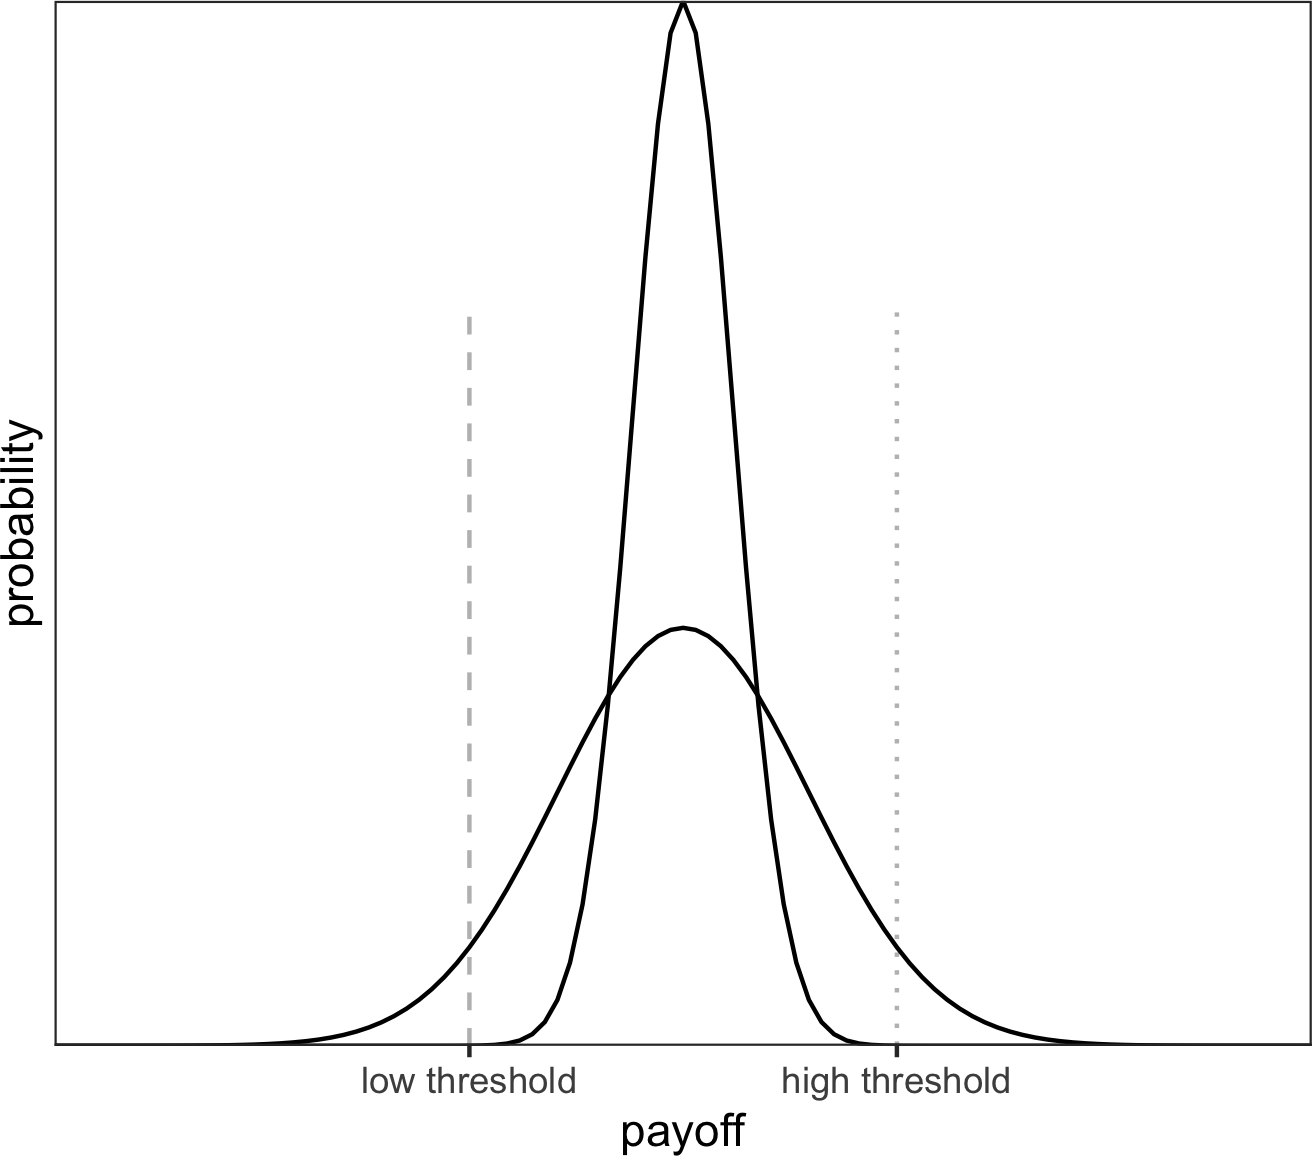
\includegraphics[width=0.6\linewidth]{rr-risk-sensitivity_files/figure-latex/varianceplot-1} 

}

\caption{Survival thresholds. When fitness drops to zero below the low threshold (dashed line), individuals should be risk-averse because the outcomes of the low-risk option (narrow distribution) are guaranteed to lie above the threshold and the outcomes of the high-risk option (wide distribution) have a non-negligible risk of falling below the threshold. When fitness drops to zero below the high threshold (dotted line), individuals should be risk-prone because only the high-risk option provides a chance of passing the threshold.}\label{fig:varianceplot}
\end{figure}

\hypertarget{survival-thresholds-and-competition}{%
\paragraph{Survival thresholds and competition}\label{survival-thresholds-and-competition}}

A final important factor for risk-sensitive behaviour are thresholds for survival and reproduction (Hurly, 2003; Winterhalder et al., 1999).
Survival thresholds are cutoff points below which an individual's fitness drops to zero, for example due to starvation.
Risk-sensitivity theory predicts that an individual will be risk averse when the resources provided by a low-variance option are sufficient to meet the threshold and risk-prone when they are not (Mishra, 2014).
For example, a hummingbird that needs to acquire a certain amount of calories to survive the night will prefer a low-risk food source if the expected amount of calories is above the threshold, but avoid the low-risk source if only a higher-risk source provides a chance of survival.
One such situation is depicted in Figure~\ref{fig:varianceplot}.

Although comparable cutoff points in academic careers may have somewhat less severe consequences, they certainly exist:
The number and impact of a researcher's publications are often explicit criteria in decisions that are central to the individual's career, such as whether they will be awarded a PhD, whether they will receive grant funding, whether they will be offered a tenure-track position, or whether they will be granted tenure.
In some of these situations, the cutoff points are absolute and thus resemble survival thresholds in the biological sense, for example PhD regulations that determine a minimal number of peer-reviewed publications for a candidate to be awarded with a doctorate, or tenure contracts that specify minimal publication targets.
In other situations, the cutoff points are relative and depend on the number of eligible candidates, for example when grant funding is awarded to the 10 highest-ranked research proposals or a job is offered to the best candidate from a pool of applicants.
In cases like these, one individual's success diminishes the chances of another --- they represent \emph{competition}.
In the following, survival thresholds and competition will be treated as separate concepts to examine their differential effects on researchers' publication behaviour.

Each of the risk-relevant factors described above\(\,\)---\(\,\)non-linear fitness functions, empirical pace, survival thresholds, and competition\(\,\)---\(\,\)likely impacts researchers' decision strategies, including their choices between low-risk and high-risk publication options.
To better understand when a low-risk option like Registered Reports should be particularly attractive or unattractive, we examine the individual and interactive effects of these factors in a simulation model.

\hypertarget{simulation-model}{%
\section{Simulation model}\label{simulation-model}}

We develop an evolutionary agent-based model which simulates a population of researchers who test hypotheses, (attempt to) publish the results either as Registered Reports or as standard reports, accumulate the payoffs for successful publications, and pass their publication strategies on to the next generation of researchers.

\hypertarget{research-phase}{%
\paragraph{Research phase}\label{research-phase}}

Consider a population of \(n = 500\) researchers.
Each researcher has a fixed publication strategy \(s\), the so-called submission threshold.
In each round of the research phase, researchers randomly choose a hypothesis to test in a study.
Hypotheses are true with prior probability \(p\), which is uniformly distributed between 0 and 1 and known to the researcher.
Before testing their chosen hypothesis, a researcher compares the prior \(p\) of their hypothesis with their publication strategy \(s\).
When \(p < s\), the researcher chooses to play it safe and conduct a Registered Report to test the hypothesis.
When \(p \geq s\), the researcher chooses to gamble and test the hypothesis in a regular study which is then submitted as a standard report.

For simplicity, we assume that \(p\) is an ideal objective prior and that researchers' hypothesis tests are free from additional sources of error.
Thus, when a researcher tests hypothesis \(i\), they obtain a positive result with probability \(p_i\) and a negative result with probability \(1-p_i\).
If the researcher chose to submit a Registered Report, their study is published regardless of the result and the researcher receives a payoff \(b_{RR}\).
However, if the researcher chose to submit a standard report, they face rampant publication bias:
Only positive results are publishable as standard reports and yield a payoff \(b_{SR+} = 1\), whereas negative results are rejected or file-drawered and yield no payoff, \(b_{SR-} = 0\).
For all variations of the model tested here, we assume that the payoff for a Registered Report falls between these bounds, such that \(b_{SR-} < b_{RR} < b_{SR+}\).
This assumption reflects the following considerations:

\begin{enumerate}
\def\labelenumi{\arabic{enumi}.}
\tightlist
\item
  Due to publication bias in the standard literature, negative results are less valuable than positive results (\(b_{SR-} < b_{SR+}\)), for example because they do not lead to a publication at all, because only very low-impact journals are willing to publish them, or because getting them published requires a lot of extra effort (e.g., via frequent resubmissions following rejection or substantial revisions demanded by reviewers), which diminishes the net reward.
\item
  For these same reasons, Registered Reports are on average more valuable than standard reports with negative results (\(b_{SR-} < b_{RR}\)), for example because Registered Reports are offered by journals that may display publication bias for standard reports (rejecting standard report submissions with negative results), or simply because Registered Reports need to be resubmitted less often or require less extensive revisions.
\item
  On average, standard reports with positive results are more valuable than Registered Reports (\(b_{RR} < b_{SR+}\)), for example because many high-impact journals do not (yet) offer Registered Reports, because not registering one's study \emph{a priori} makes it easier to spin the results to appear more impactful and thus increases the chances to be published in a high-impact journal, or because Registered Reports may require more effort due to their stricter quality criteria, lowering the net reward.
  While proponents of Registered Reports may argue that the format has such tremendous advantages that authors' resulting career benefits are superior to any alternative, this chapter is predicated on the assumption that most researchers currently do not share this view.
  Once this changes, the present investigation may happily become redundant.
\end{enumerate}

This entire research cycle\(\,\)---\(\,\)choosing a hypothesis, choosing a publication route by comparing its prior \(p\) to one's publication strategy \(s\), testing the hypothesis, and receiving payoff \(b_{RR}\) for a Registered Report or \(b_{SR-}\) or \(b_{SR+}\) for a positive and negative standard report, respectively\(\,\)---\(\,\)is repeated \(m\) times.

\hypertarget{evaluation-phase}{%
\paragraph{Evaluation phase}\label{evaluation-phase}}

At the end of the research phase, researchers' accumulated publication payoffs \(b_1 + b_2 + ... + b_m\) are translated into fitness \(f\).
Fitness is calculated with a function characterised by exponent \(\epsilon\), which determines the shape of the function. \(\epsilon = 1\) yields a linear function, \(0 < \epsilon < 1\) yields a concave function with diminishing returns, and \(\epsilon > 1\) yields a convex function with increasing returns (see Figure~\ref{fig:fitnessplot}):

\begin{align}
f = (\sum_{i=1}^{m} b_i)^\epsilon
\end{align}

However, two situations may cause a researcher's fitness to fall to zero even when their accumulated payoffs are non-zero.
First, the sum of their payoffs may fall below an absolute survival threshold \(\delta\), for example when a researcher fails to meet an agreed publication target by the time their `tenure clock' runs out.
Thus, when \(\sum_{i=1}^{m} b_i < \delta\), \(f = 0\).
Second, the sum of their payoffs may fall below a relative threshold \(\gamma\), which reflects the intensity of competition (e.g., for scarce research grants or positions).
\(\gamma\) is the proportion of researchers who are considered for reproduction.
When \(\gamma = 1\), all researchers in the population are considered for reproduction and their fitness is calculated according to Eq. 1.
When \(\gamma < 1\), the \((1 - \gamma)*500\) least successful researchers receive zero fitness and cannot reproduce.\footnote{In the simulation, \(\gamma\) is applied \emph{after} fitness has been calculated, not before. This change has purely technical reasons and leads to the same result as applying \(\gamma\) to accumulated payoffs and then calculating fitness because all fitness functions are monotonic increasing and fitness functions do not vary within a population. That is, applying the fitness function does not affect the rank order of researchers in the population.}
For example, \(\gamma = 0.1\) means that only those researchers with accumulated payoffs in the top \(10\%\) of the population can reproduce, and the fitness of the remaining \(90\%\) is set to zero.

\begin{longtable}[]{@{}
  >{\centering\arraybackslash}p{(\columnwidth - 4\tabcolsep) * \real{0.1273}}
  >{\raggedright\arraybackslash}p{(\columnwidth - 4\tabcolsep) * \real{0.6364}}
  >{\raggedright\arraybackslash}p{(\columnwidth - 4\tabcolsep) * \real{0.2364}}@{}}
\caption{Parameter definitions and values}\tabularnewline
\toprule()
\begin{minipage}[b]{\linewidth}\centering
Parameter
\end{minipage} & \begin{minipage}[b]{\linewidth}\raggedright
Definition
\end{minipage} & \begin{minipage}[b]{\linewidth}\raggedright
Value {[}range{]}
\end{minipage} \\
\midrule()
\endfirsthead
\toprule()
\begin{minipage}[b]{\linewidth}\centering
Parameter
\end{minipage} & \begin{minipage}[b]{\linewidth}\raggedright
Definition
\end{minipage} & \begin{minipage}[b]{\linewidth}\raggedright
Value {[}range{]}
\end{minipage} \\
\midrule()
\endhead
\(n\) & population size & 500 \\
\(g\) & number of generations & 250 \\
\(p\) & prior probability of hypotheses & uniform {[}0--1{]} \\
\(b_{SR-}\) & payoff for negative standard report & 0 \\
\(b_{SR+}\) & payoff for positive standard report & 1 \\
\(b_{RR}\) & payoff for Registered Report & {[}.1, .2, \ldots, .9{]} \\
\(\epsilon\) & fitness function exponent & {[}0.2, 1, 5{]} \\
\(m\) & research cycles per generation (`empirical pace') & {[}1, 2, 4, 8, 16, 32{]} \\
\(\delta\) & survival threshold below which fitness = 0, expressed as proportion of m & {[}0, .25, .5, .75{]} \\
\(\gamma\) & proportion of most successful researchers selected for reproduction (competition) & {[}1, .9, .5, .1, .05, .01{]} \\
\bottomrule()
\end{longtable}

\hypertarget{reproduction-phase}{%
\paragraph{Reproduction phase}\label{reproduction-phase}}

Finally, the researchers in the current population retire and a new (non-overlapping) generation of researchers is created.
A researcher in the new generation inherits their publication strategy \(s\) from a researcher in the previous generation with the probability of the previous researcher's fitness (i.e., the new generation's publication strategies are sampled with replacement from the previous generation, probability-weighted by fitness).
The new generation's publication strategies are inherited with a small amount of random noise, such that \(s_{new} = s_{old} + w\), with \(w \sim N(\mu = 0, \sigma = 0.01)\).
Authors of similar evolutionary agent-based models have described such hereditary transmission as reflecting mentorship and teaching (e.g., when established professors advise mentees to copy their strategies) or simply a generic social learning process in which successful researchers are more likely to be imitated by others (Smaldino \& McElreath, 2016).
Although this interpretation may be useful, the main purpose of this aspect of the model is purely technical and not specifically intended to reflect reality\(\,\)---\(\,\)it simply provides the machinery for determining which publication strategies are optimal in the various situations we are investigating.

\hypertarget{outcome-variable-s}{%
\subsubsection{\texorpdfstring{Outcome variable \(s\)}{Outcome variable s}}\label{outcome-variable-s}}

We study how the evolution of researchers' publication strategies \(s\) is affected by the payoff for Registered Reports \(b_{RR}\) (relative to the payoffs for standard reports, which are fixed at \(b_{SR-} = 0\) and \(b_{SR+} = 1\)), by the shape of the fitness function determined by exponent \(\epsilon\), by the number of research cycles per generation \(m\), by survival threshold \(\delta\), and by competition \(\gamma\) (see Table 1 for an overview of the model parameters and their values considered in the simulation).
It is important to keep in mind that a researcher's publication strategy \(s\) is
not an absolute decision:
It determines \emph{how} the choice between Registered Reports and standard reports is made, not which format is chosen.
As such, \(s\) indicates the amount of risk a researcher is willing to take.
Very low values of \(s\) reflect risk proneness:
The researcher prefers to gamble and chooses the standard publication route for almost all hypotheses they encounter, using the Registered Report route only for hypotheses that are virtually guaranteed to be false (and yield negative results).
Very high values of \(s\) reflect risk aversion:
The researcher is unwilling to risk a negative result in a standard report and studies almost all hypotheses they encounter in the Registered Report format, reserving the standard publication route for hypotheses that are virtually guaranteed to be true (and yield positive results).

\hypertarget{simulation-approach}{%
\subsubsection{Simulation approach}\label{simulation-approach}}

We use the evolutionary mechanism of this agent-based model as a means for identifying optimal behaviour under different conditions.
But this goal can also be achieved in other ways.
One non-evolutionary alternative is to calculate expected fitness (i.e., the long-run average) for a wide range of \(s\) and determine which strategy maximises it in each condition.
A drawback of this approach is that it does not account for population dynamics and therefore cannot easily simulate the effects of competition.
Because of this limitation, our study is based on the evolutionary model.
However, we validate all analyses except those involving competition on the expected-fitness model and show that both models produce virtually identical results (see Appendix).



\begin{figure}

{\centering 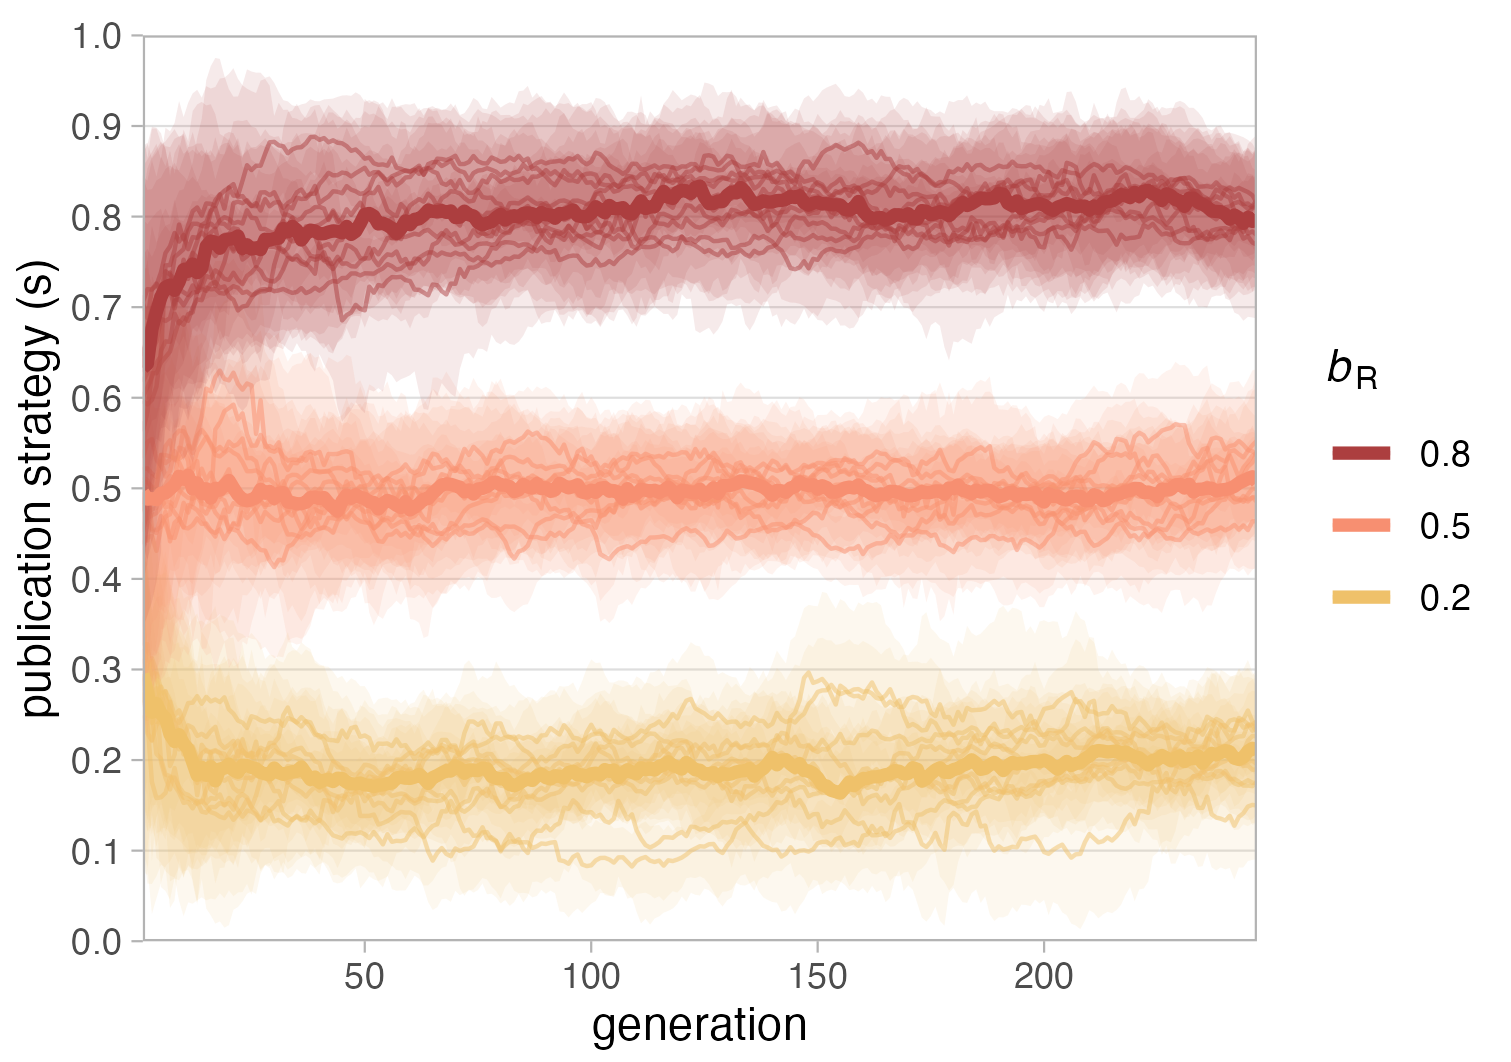
\includegraphics[width=5.04in]{plots/plot_evo} 

}

\caption{Evolution of publication strategy \(s\) with 3 different payoffs for Registered Reports (\(b_{RR}\)). Simulations are based on a population of \(n = 500\) researchers over 250 generations, with payoffs for standard reports fixed at 0 for negative results (\(b_{SR-} = 0\)) and 1 for positive results (\(b_{SR+} = 1\)), a linear fitness function \(\epsilon = 1\), one research cycle per generation (\(m = 1\)), no survival threshold (\(\delta = 0\)) and no competition (\(\gamma = 1\)). Each condition was run 10 times. Thin lines represent the median publication strategy of the population in each run, shaded areas represent the inter-quartile range of publication strategies in the population in each run, and thick lines represent the median of run medians per condition.}\label{fig:evoplot}
\end{figure}

\hypertarget{simulation-results}{%
\section{Simulation results}\label{simulation-results}}

The results of the simulation models will be presented in order of increasing model complexity.
We start by explaining the very simple scenarios shown in Figure \ref{fig:evoplot} and Figure \ref{fig:epsilonplot}.
These scenarios are identical to situations discussed above and the results should thus be unsurprising.
However, while they may seem trivial to some, we hope that these explanations will help unfamiliar readers understand the basic functioning of our model as well as the less intuitive results presented later.

When interpreting the results below, one should bear in mind that the analysed parameter values are inherently arbitrary.
Although the model parameters are intended to capture important characteristics of real-world concepts, their values do not represent real-world units.
The goal of this analysis is to understand the relative effects of the model parameters in a simplified, artificial system, which means that the results are only meaningful in relation to each other.

\hypertarget{single-research-cycle-per-generation-linear-fitness-function}{%
\subsection{Single research cycle per generation, linear fitness function}\label{single-research-cycle-per-generation-linear-fitness-function}}

The first generation of researchers in each simulation run is initialised with randomly distributed publication strategies \(s\) (drawn from a uniform distribution {[}0--1{]}), which are then allowed to evolve over the subsequent generations.
Figure \ref{fig:evoplot} shows the effect of varying the payoffs for Registered Reports when the fitness function is linear (\(\epsilon = 1\)), with no survival threshold (\(\delta = 0\)), no competition (\(\gamma = 1\)), and one research cycle per generation (\(m = 1\)).
In this very simple scenario, evolved publication strategies (\(s\)) approximate the payoff for Registered Reports in each condition, indicating that the optimal publication strategy is always equal to \(b_{RR}\) (\(s_{optimal} = 0.2\) when \(b_{RR} = 0.2\), \(s_{optimal} = 0.5\) when \(b_{RR} = 0.5\), \(s_{optimal} = 0.8\) when \(b_{RR} = 0.8\)).
The reason behind this is the uniform distribution {[}0--1{]} of hypothesis priors, the payoff structure \(b_{SR-} = 0\) and \(b_{SR+} = 1\), and the linear fitness function (\(\epsilon = 1\) means that fitness equals payoff).
In this constellation, the expected fitness obtained from a standard report is always equal to the prior of the tested hypothesis:

\begin{align}
E[f_{SR}] = (p * b_{SR+} + (1-p) * b_{SR-})^1 = p * 1 +  (1-p) * 0 = p
\end{align}

For example, testing a hypothesis with \(p = 0.2\) in a standard report would yield the expected fitness \(E[f_{SR}] = (0.2 * 1 + 0.8 * 0)^1 = 0.2\).
The optimal strategy is to submit a Registered Report whenever the expected fitness provided by a standard report is lower than the fitness provided by a Registered Report, \(E[f_{SR}] < b_{RR}\), and thus whenever \(p < b_{RR}\).
This ensures that researchers always get the best of both worlds, minimising shortfalls when priors are (too) low and maximising winning chances when priors are (sufficiently) high.
For example, \(b_{RR} = 0.5\) is larger than \(E[f_{SR}]\) for all hypotheses with \(p < 0.5\) but smaller than \(E[f_{SR}]\) for all hypotheses with \(p > 0.5\).
In this situation, researchers who submit Registered Reports whenever \(p<0.5\) and standard reports whenever \(p>0.5\) protect themselves against losing a bad bet by instead taking the fixed payoff \(b_{RR} = 0.5\), but always play a good bet and thus maximise their chances of winning \(b_{SR+} = 1\).
Every alternative is inferior in the long run because researchers with \(s > b_{RR}\) lose out on increased chances of publishing a standard report and researchers with \(s < b_{RR}\) take unnecessary risks and go empty-handed too often.



\begin{figure}

{\centering 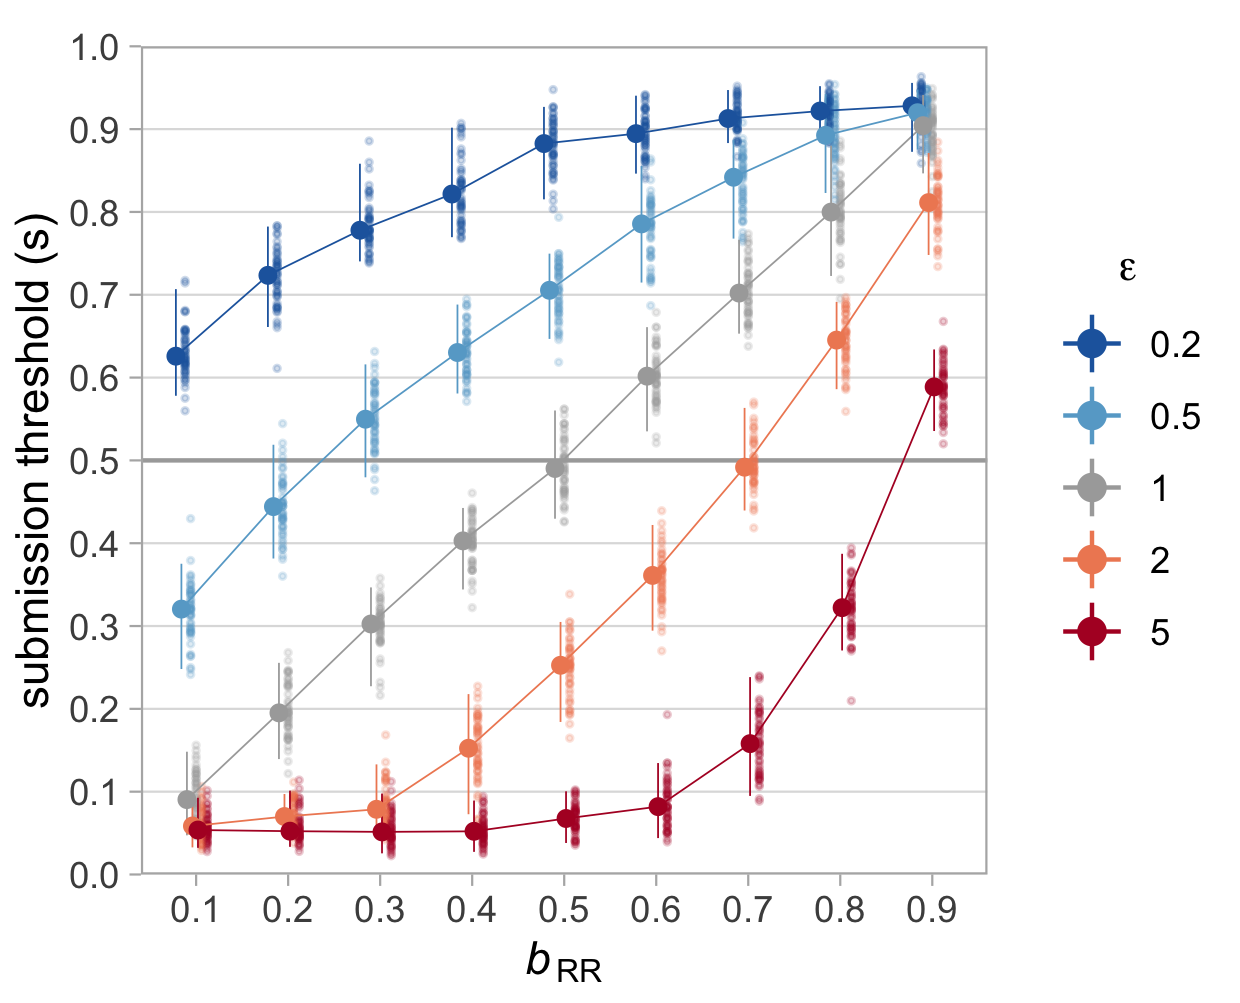
\includegraphics[width=0.65\linewidth]{plots/plot_b_epsilon} 

}

\caption{Effect of fitness functions on evolved publication strategies. Shown are median publication strategies in the final (\(250^{th}\)) generations of 50 runs for different values of \(b_{RR}\) (x-axis) and different fitness functions (characterised by exponent \(\epsilon\)), with one research cycle per generation (\(m = 1\)), no survival threshold (\(\delta = 0\)) and no competition (\(\gamma = 1\)). Fitness functions with \(\epsilon = 0.2\) and \(\epsilon = 0.5\) (blue lines) are concave with diminishing returns, functions with \(\epsilon = 2\) and \(\epsilon = 5\) (red lines) are convex with increasing returns, and the function with \(\epsilon = 1\) (grey line) is linear. Small dots represent median \(s\) of the final generation in each run, large dots represent the median of these 50 run medians per condition. Error bars represent the \(95\%\) capture probability around the median of medians.}\label{fig:epsilonplot}
\end{figure}

\hypertarget{allowing-for-non-linear-fitness-functions}{%
\subsection{Allowing for non-linear fitness functions}\label{allowing-for-non-linear-fitness-functions}}

Arguably, the career benefits researchers receive from publications in the real world are rarely, if ever, linear.
In early career, we may assume a convex fitness function, with each addition to the short publication record of a young researcher yielding increasing returns for their prospects on the job market and their ability to obtain grant funding.
A notable exception may be PhD students who plan to leave academia after obtaining their degree, and for whom the career returns of publications exceeding the PhD requirements are thus strongly decreasing (concave fitness function).
Researchers who stay in academia may experience that the career returns for each additional publication begin to decrease as their publication record grows, meaning that advanced career stages may also be characterised by a concave fitness function.

Figure \ref{fig:epsilonplot} contrasts the effects of two concave fitness functions (\(\epsilon = 0.2\) and \(\epsilon = 0.5\), shown in blue shades) and two convex fitness functions (\(\epsilon = 2\) and \(\epsilon = 5\), shown in red shades) with a linear function (\(\epsilon = 1\), grey line) for different payoffs for Registered Reports, in the same simple scenario with only one research cycle per generation.
The grey line for \(\epsilon = 1\) represents the already familiar situation from Figure \ref{fig:evoplot} above:
When the fitness function is linear, the optimal strategy is \(s_{optimal} = b_{RR}\).
Non-linear fitness functions deviate from this pattern exactly as expected based on Figure \ref{fig:fitnessplot}.
When additional payoffs yield diminishing returns (\(\epsilon <1\)), Registered Reports become more attractive even when they are worth less than the expected payoff for standard reports.
As explained above, this is because concave functions `shrink' the difference between moderate and high payoffs relative to the difference between low and moderate payoffs.
Conversely, when additional payoffs yield increasing returns (\(\epsilon > 1\)), Registered Reports are unattractive unless their payoffs are almost as large as those for published standard reports because convex functions increase the difference between moderate and high payoffs relative to low versus moderate payoffs.

When different fitness functions are taken to reflect different career stages,
this pattern suggests that Registered Reports should be more attractive for senior researchers and a tough sell for early-career researchers.
Interestingly, preliminary empirical evidence suggests the opposite:
Registered Reports appear to be more likely to have early-career researchers as first authors than standard reports (77\% vs 67\% in the journal \emph{Cortex}, Chambers \& Tzavella, 2022).
One explanation for this counterintuitive result could be that Registered Reports are disproportionally used by early-career researchers who intend to leave academia and thus have a concave fitness function.
Alternatively, factors or dynamics not considered in this simulation may swamp out the effects of concave \emph{vs} convex fitness functions, such as younger researchers being more likely to adopt new methods.
However, as we will see below, the effects of different fitness functions are not always as straightforward as in the simple case illustrated in Figure \ref{fig:epsilonplot} but produce different results in interaction with other risk-related factors.



\begin{figure}

{\centering 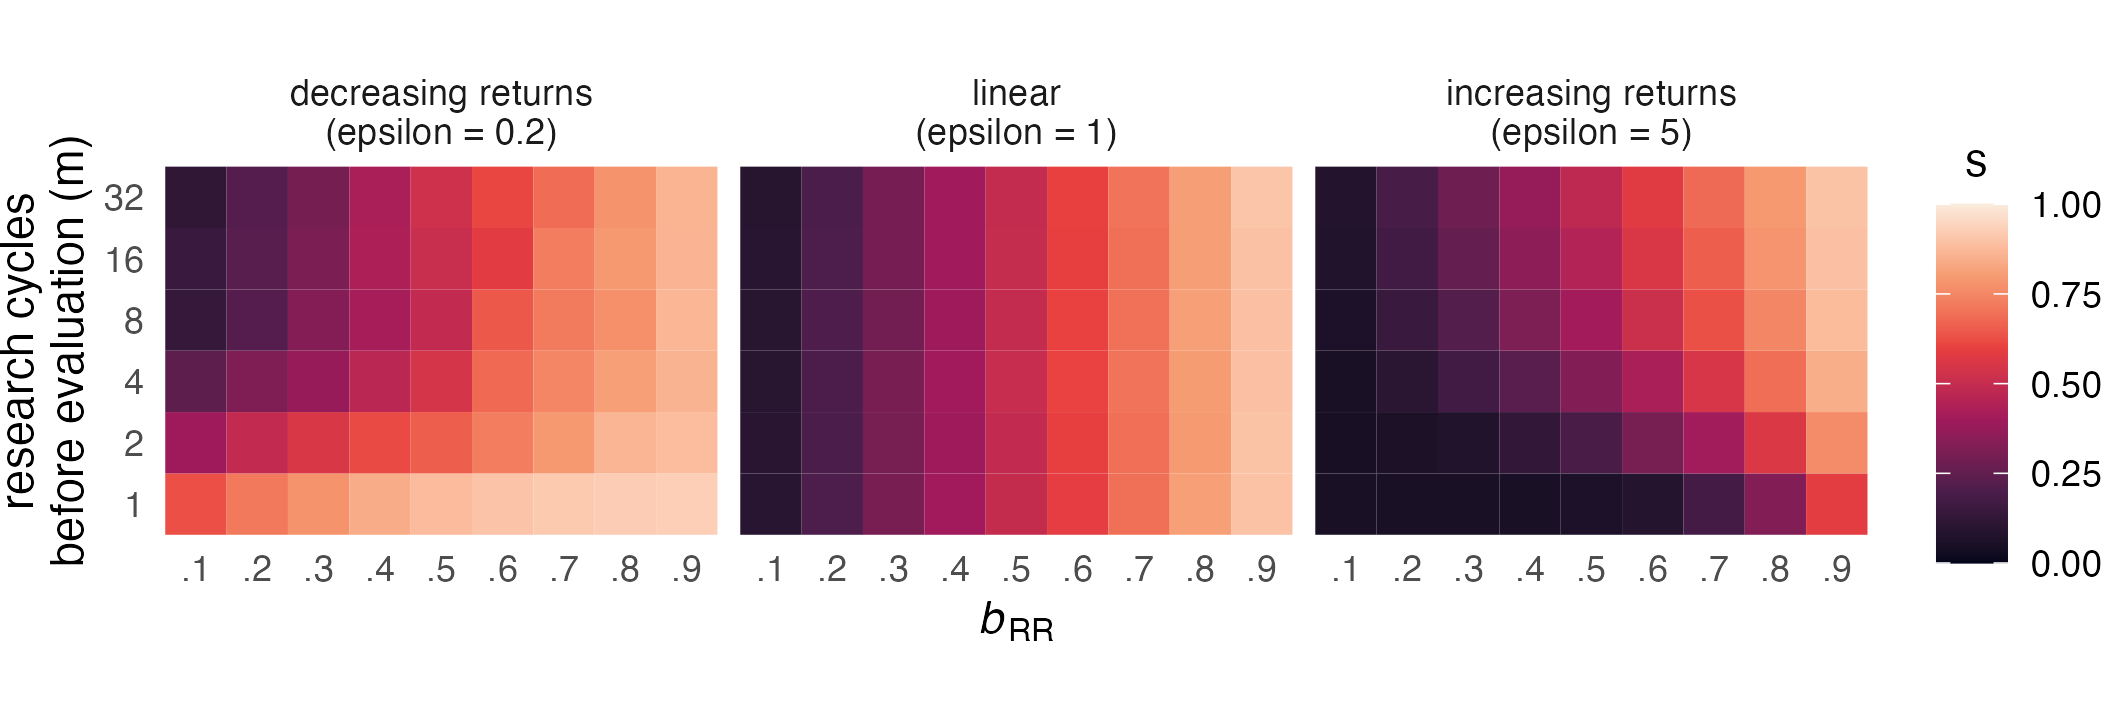
\includegraphics[width=1\linewidth]{plots/plot_m_evo_rocket} 

}

\caption{Effect of research cycles per generation on evolved publication strategies. Shown are median evolved publication strategies (\(s\)) after 250 generations in 50 runs (tile colour represents the median of 50 run medians) depending on the number of research cycles per generation (\(m\), y-axis), different values of \(b_{RR}\) (x-axis), and different fitness functions (characterised by exponent \(\epsilon\)) with no survival threshold (\(\delta = 0\)) and no competition (\(\gamma = 1\)).}\label{fig:mplot}
\end{figure}

\hypertarget{varying-the-number-of-research-cycles-per-generation}{%
\subsection{Varying the number of research cycles per generation}\label{varying-the-number-of-research-cycles-per-generation}}

The analyses presented so far focused on the simple case of one research cycle (or decision event) per generation, meaning that researchers' fitness was calculated based on the payoff from one single study.
As discussed above, increasing numbers of decision events prior to evaluation may make individuals more risk-prone because single negative outcomes are less catastrophic for reproduction (Haaland et al., 2019).
However, Figure \ref{fig:mplot} shows that this is not universally true\(\,\)---\(\,\)rather, the effect of increasing numbers of research cycles per generation (\(m\)) depends on the shape of the fitness function.
Moving up on the y-axis of each panel, we see that \(s\) decreases (indicating greater risk proneness) only when the fitness function is concave (\(\epsilon = 0.2\), left panel) but stay constant when it is linear (\(\epsilon = 1\), middle panel) and even \emph{increases} when it is convex (\(\epsilon = 5\), right panel).

Why does \(m\) appear to have opposite effects for concave and convex fitness functions?
As a starting point, it helps to first consider only the bottom row of each panel, where \(m = 1\).
These three rows contain the same results as the top, middle, and bottom curves in Figure \ref{fig:epsilonplot} and show risk aversion when \(\epsilon = 0.2\) (i.e., Registered Reports are attractive even when they yield a low payoff), risk proneness when \(\epsilon = 5\) (Registered Reports are unattractive even when they yield a high payoff), and a linear strategy \(s_{optimal} = b_{RR}\) when \(\epsilon = 1\).
From this starting point, the two panels with non-linear fitness functions start to approximate the linear case as \(m\) increases.
This pattern reflects the idea that fitness is better captured by the geometric mean when \(m\) is low, and better captured by the arithmetic mean when \(m\) is high (Haaland et al., 2019).

To better understand this dynamic, let's consider two researchers with extreme submission strategies:
Regina Register conducts only Registered Reports (\(s_{Regina} = 1\)), Darren Daring conducts only standard reports (\(s_{Darren} = 0\)).
The payoff for Registered Reports is fixed at \(b_{RR} = 0.5\).
After one research cycle, Regina receives a payoff of 0.5 and Darren receives either 0 or 1 (with 50/50 odds).
If fitness is calculated after this one round with \(\epsilon = 0.2\) (concave function, yielding diminishing returns), Regina's fitness is \(f_{Regina} = \frac{1}{2}^{\frac{1}{5}} = 0.87\), and Darren's fitness is either \(f_{Darren-} = 0^{\frac{1}{5}} = 0\) or \(f_{Darren+} = 1^{\frac{1}{5}} = 1\).
In a population of 100 Reginas and 100 Darrens, there will be roughly 50 lucky Darrens who get a positive result and 50 Darrens who get a negative result.
Lucky Darrens have a narrow fitness advantage over all Reginas (1 versus 0.87), while unlucky Darrens lose to all Reginas by a wide margin (0 versus 0.87).
Since there are twice as many Reginas as lucky Darrens, the Regina strategy is relatively more successful.

Let's now consider the same scenario with \(m = 4\) research cycles per generation.
Reginas receive the same payoff in every round and accumulate \(b_{total} = \frac{1}{2} * 4 = 2\).
Lucky Darrens (who win every time) accumulate \(b_{total} = 1*4 = 4\), while unlucky Darrens (who lose every time) again receive 0 total payoff.
Now, however, the probabilistic outcomes over 4 rounds lead to three additional versions of Darren: moderately lucky (winning 3/4 times), average (2/4, receiving the same total payoff as Reginas), and moderately unlucky (1/4).
Translating payoffs into fitness, the Regina strategy (\(f_{Regina} = 2^\frac{1}{5} = 1.15\)) still yields an enormous advantage compared to unlucky Darrens (\(f_{Darren_{unlucky}} = 0\)) and only a small disadvantage compared to lucky Darrens (\(f_{Darren_{lucky}} = 4^\frac{1}{5} = 1.32\)).
But this time, there are fewer Darrens who are less successful than Reginas because Reginas now share their place with average Darrens.
The relative fitness advantage of the Regina strategy thus decreases.
As the rate of research cycles per generation grows, the law of large numbers dictates that more and more Darrens achieve average total payoffs, while fewer and fewer Darrens achieve extreme total payoffs (winning 32 times in a row is much less probable than winning 4 times in a row).
This reduces the width of the Darren distribution until it approximates the Regina distribution\(\,\)---\(\,\)meaning that optimal publication strategies become identical to those optimal for a linear fitness function.

When the fitness function is convex (\(\epsilon = 5\), yielding increasing returns), the overall effect of increasing values of \(m\) is the same, with the only difference that Reginas are initially disadvantaged (because their fitness distance to the lucky half of Darrens is much greater than than to the unlucky Darrens).
With larger \(m\), more and more Darrens receive average total payoffs and share Regina's disadvantaged position (decreasing Regina's relative disadvantage), until the Darren distribution is again virtually equal to the Regina distribution.
Rather than causing absolute risk aversion, increasing values of \(m\) thus counter the effect of \(\epsilon\) and reduce the effects of concave and convex fitness functions to the linear case.
Consequently, the top rows (\(m = 32\)) of the top and bottom panels in Figure \ref{fig:mplot} resemble the stable pattern across all \(m\) shown in the middle panel.

Translated into terms of academic careers, this less intuitive pattern indicates that
being able to complete empirical studies at a higher rate\(\,\)---\(\,\)e.g., when working in a field where data collection is fast and cheap or when having more resources for data collection available\(\,\)---\(\,\)may cancel out the effects of different career stages.
This could partly explain why Registered Reports appear to be less popular among senior researchers (Chambers \& Tzavella, 2022) than we would expect based on the effects of different fitness functions alone:
Although additional publications likely yield diminishing returns in later career stages (concave fitness function), academic seniority often comes with resources that boost research output per time (e.g., more lab members).
As a consequence, established professors may be relatively indifferent to Registered Reports.
Regarding junior researchers (for whom additional publications have increasing returns on career success), the results suggest that they may be especially reluctant to use Registered Reports when they have very limited time or resources to produce publications before an important selection event, such as on short-term postdoc contracts (R. Müller \& de Rijcke, 2017).



\begin{figure}
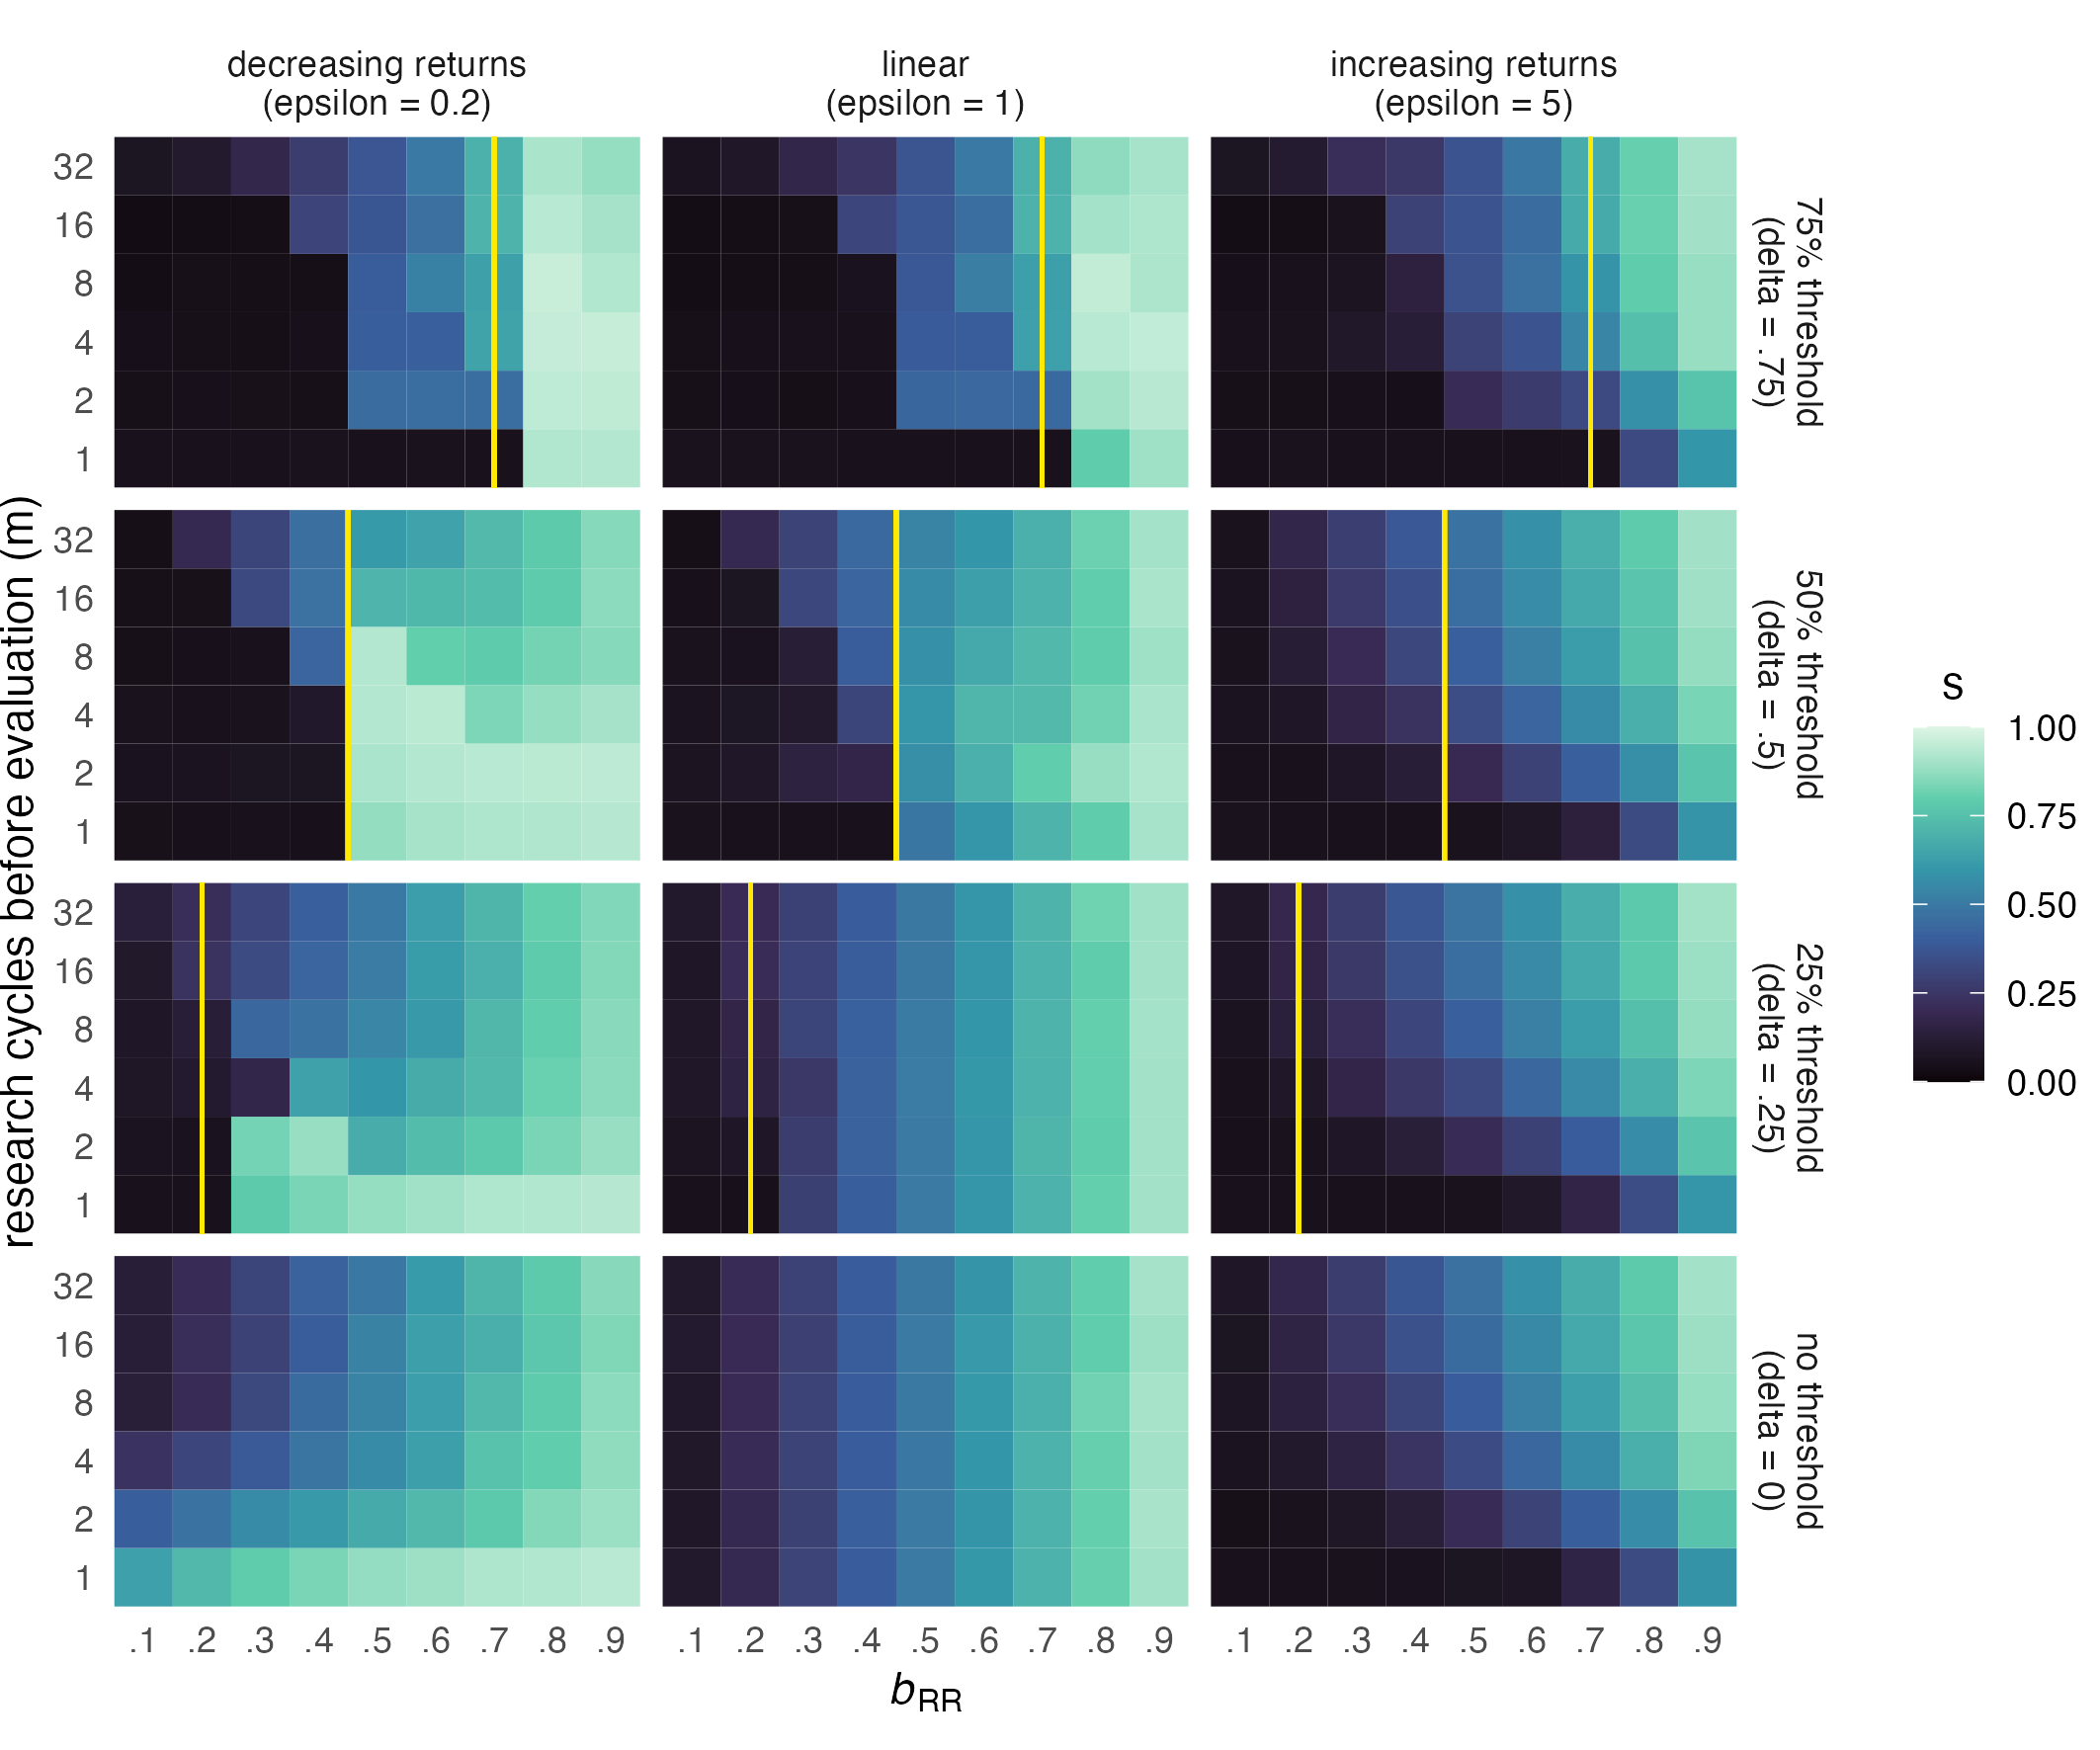
\includegraphics[width=1\linewidth]{plots/plot_delta_tile_evo_epsilon_mako} \caption{Effect of survival thresholds on evolved publication strategies. Shown are median publication strategies (\(s\)) after 250 generations in 50 runs (tile colour represents the median of 50 run medians) depending on survival thresholds (\(\delta\), shown as vertical yellow line), fitness functions (characterised by exponent \(\epsilon\)), numbers of research cycles per generation (\(m\)), and values of \(b_{RR}\), in the absence of competition (\(\gamma = 1\)). Survival thresholds are set as proportions of \(m\), i.e., as a percentage of the maximum possible payoff in each condition. To reproduce, researchers must accumulate a total payoff exceeding \(\delta * m\).}\label{fig:deltaplot}
\end{figure}

\hypertarget{absolute-survival-thresholds}{%
\subsection{Absolute survival thresholds}\label{absolute-survival-thresholds}}

The survival thresholds (\(\delta\)) in our model represent absolute publication targets that researchers must meet in order to progress in their career.
The clearest examples for such thresholds are PhD regulations and tenure agreements.
To be awarded with a PhD, many institutions and faculties require candidates to have a certain number of their thesis chapters published in peer-reviewed journals.
Similarly, tenure agreements may include publication targets in the form of a minimum number of peer-reviewed publications within a certain time, sometimes also specifying minimal journal ranks (Liner \& Sewell, 2009).
Such requirements may represent low, medium, or high survival thresholds depending on how demanding they are (e.g., the proportion of thesis chapters that must be published).

We investigate the effects of survival thresholds representing 25\%, 50\%, and 75\% of the maximum possible payoff researchers can achieve in one generation.
When \(\delta > b_{RR}\), Registered Reports alone are not sufficient to reach the survival threshold (\(b_{RR}\) values to the left of the yellow line in Figure \ref{fig:deltaplot}).
For example, at \(m = 4\), a survival threshold of 75\% (\(\delta = .75\)) means that researchers must gain at least 3 points to be able to reproduce.
When \(b_{RR} = .7\), submitting four Registered Reports will only amount to 2.8 points in total, just short of meeting the threshold.
On the other hand, when \(b_{RR} = .8\) (i.e., just above \(\delta\)), four Registered Reports would yield 3.2 points and thus ensure reproduction.
Choosing the standard route some of the time can increase fitness even further, but also increases the risk of not meeting the survival threshold.
As a consequence, one may intuitively expect Registered Reports to be popular whenever \(\delta \leq b_{RR}\) and unpopular whenever \(\delta > b_{RR}\).

Figure \ref{fig:deltaplot} shows that this is true in many, but not all conditions.
First, we can see that survival thresholds have their biggest effect when the number of research cycles per generation is low\(\,\)---\(\,\)at high values of \(m\), publication strategies are virtually unaffected in all conditions.
Second, survival thresholds have a stronger effect when the fitness function is linear (\(\epsilon = 1\)) or concave (\(\epsilon = 0.2\)).
In these two conditions, they produce very similar patterns:
The Registered Report route is almost never chosen when \(b_{RR}\) is too low to meet the survival threshold (particularly at \(\delta = .25\) and \(\delta = .5\); less so at \(\delta = .75\)), and this effect tapers off as the number of research cycles increases.
Compared to baseline, the change is particularly striking for the concave fitness function (\(\epsilon = 0.2\), left column in Fig. \ref{fig:deltaplot}), where RRs are normally preferred at low \(m\).
When the survival threshold is high (\(\delta = .75\)) or the fitness function is concave, we can also see that Registered Reports become \emph{more} popular than baseline when they are worth just enough to pass the survival threshold.
For the convex fitness function (\(\epsilon = 5\)) on the other hand, survival thresholds of 25\% and 50\% seem to have no effect at all.
Only a high threshold of 75\% makes RRs even less popular when they have low value (\(b_{RR}\leq 0.4\)), especially when the number of research cycles is low.

What does this mean in practice?
In our model, fitness (according to the three different fitness functions) is calculated after the survival threshold has been met.
This is meant to mimic publication requirements that are expressed in raw numbers.
Importantly, it also means that our simulation shows which strategies during a PhD or on the tenure track lead to maximal fitness \emph{after} researchers have successfully obtained their PhD or have been granted tenure.
With this in mind, it becomes easier to understand the meaning of the different fitness functions.
As discussed above, PhD candidates plausibly receive increasing returns for additional publications (convex fitness function), unless they intend not to stay in academia, in which case returns are strongly decreasing (concave fitness function).
For researchers on the tenure track, the fitness function after achieving tenure is also likely concave, assuming a) that achieving tenure is one of the most important career goals for many (making further progress relatively less important) and b) that such individuals have already built up substantial publication records, to which any single addition makes less and less of a difference.
However, exceptions from this scenario may well exist, for example in situations where tenured researchers are under great pressure to obtain grant funding.

Translated to real-world scenarios, our results thus suggest the following implications:
First, survival thresholds are almost irrelevant when
researchers can complete large numbers of studies before they are evaluated (reflecting characteristics of the research field, available resources, or length of the evaluation period).
Second, researchers with a convex fitness function\(\,\)---\(\,\)such as PhD candidates who are pursuing an academic career\(\,\)---\(\,\)are only affected by high survival thresholds, which lead them to choose Registered Reports even less often than normal when their value is low.
Third, researchers with a concave fitness function\(\,\)---\(\,\)such as tenure candidates or PhD students who aim for careers outside of academia\(\,\)---\(\,\)are highly sensitive to the value of Registered Reports:
They virtually never conduct Registered Reports when their value is too low for meeting the survival threshold, but strongly prefer them when their value is sufficient (especially when empirical pace is low and/or the survival threshold is high).



\begin{figure}
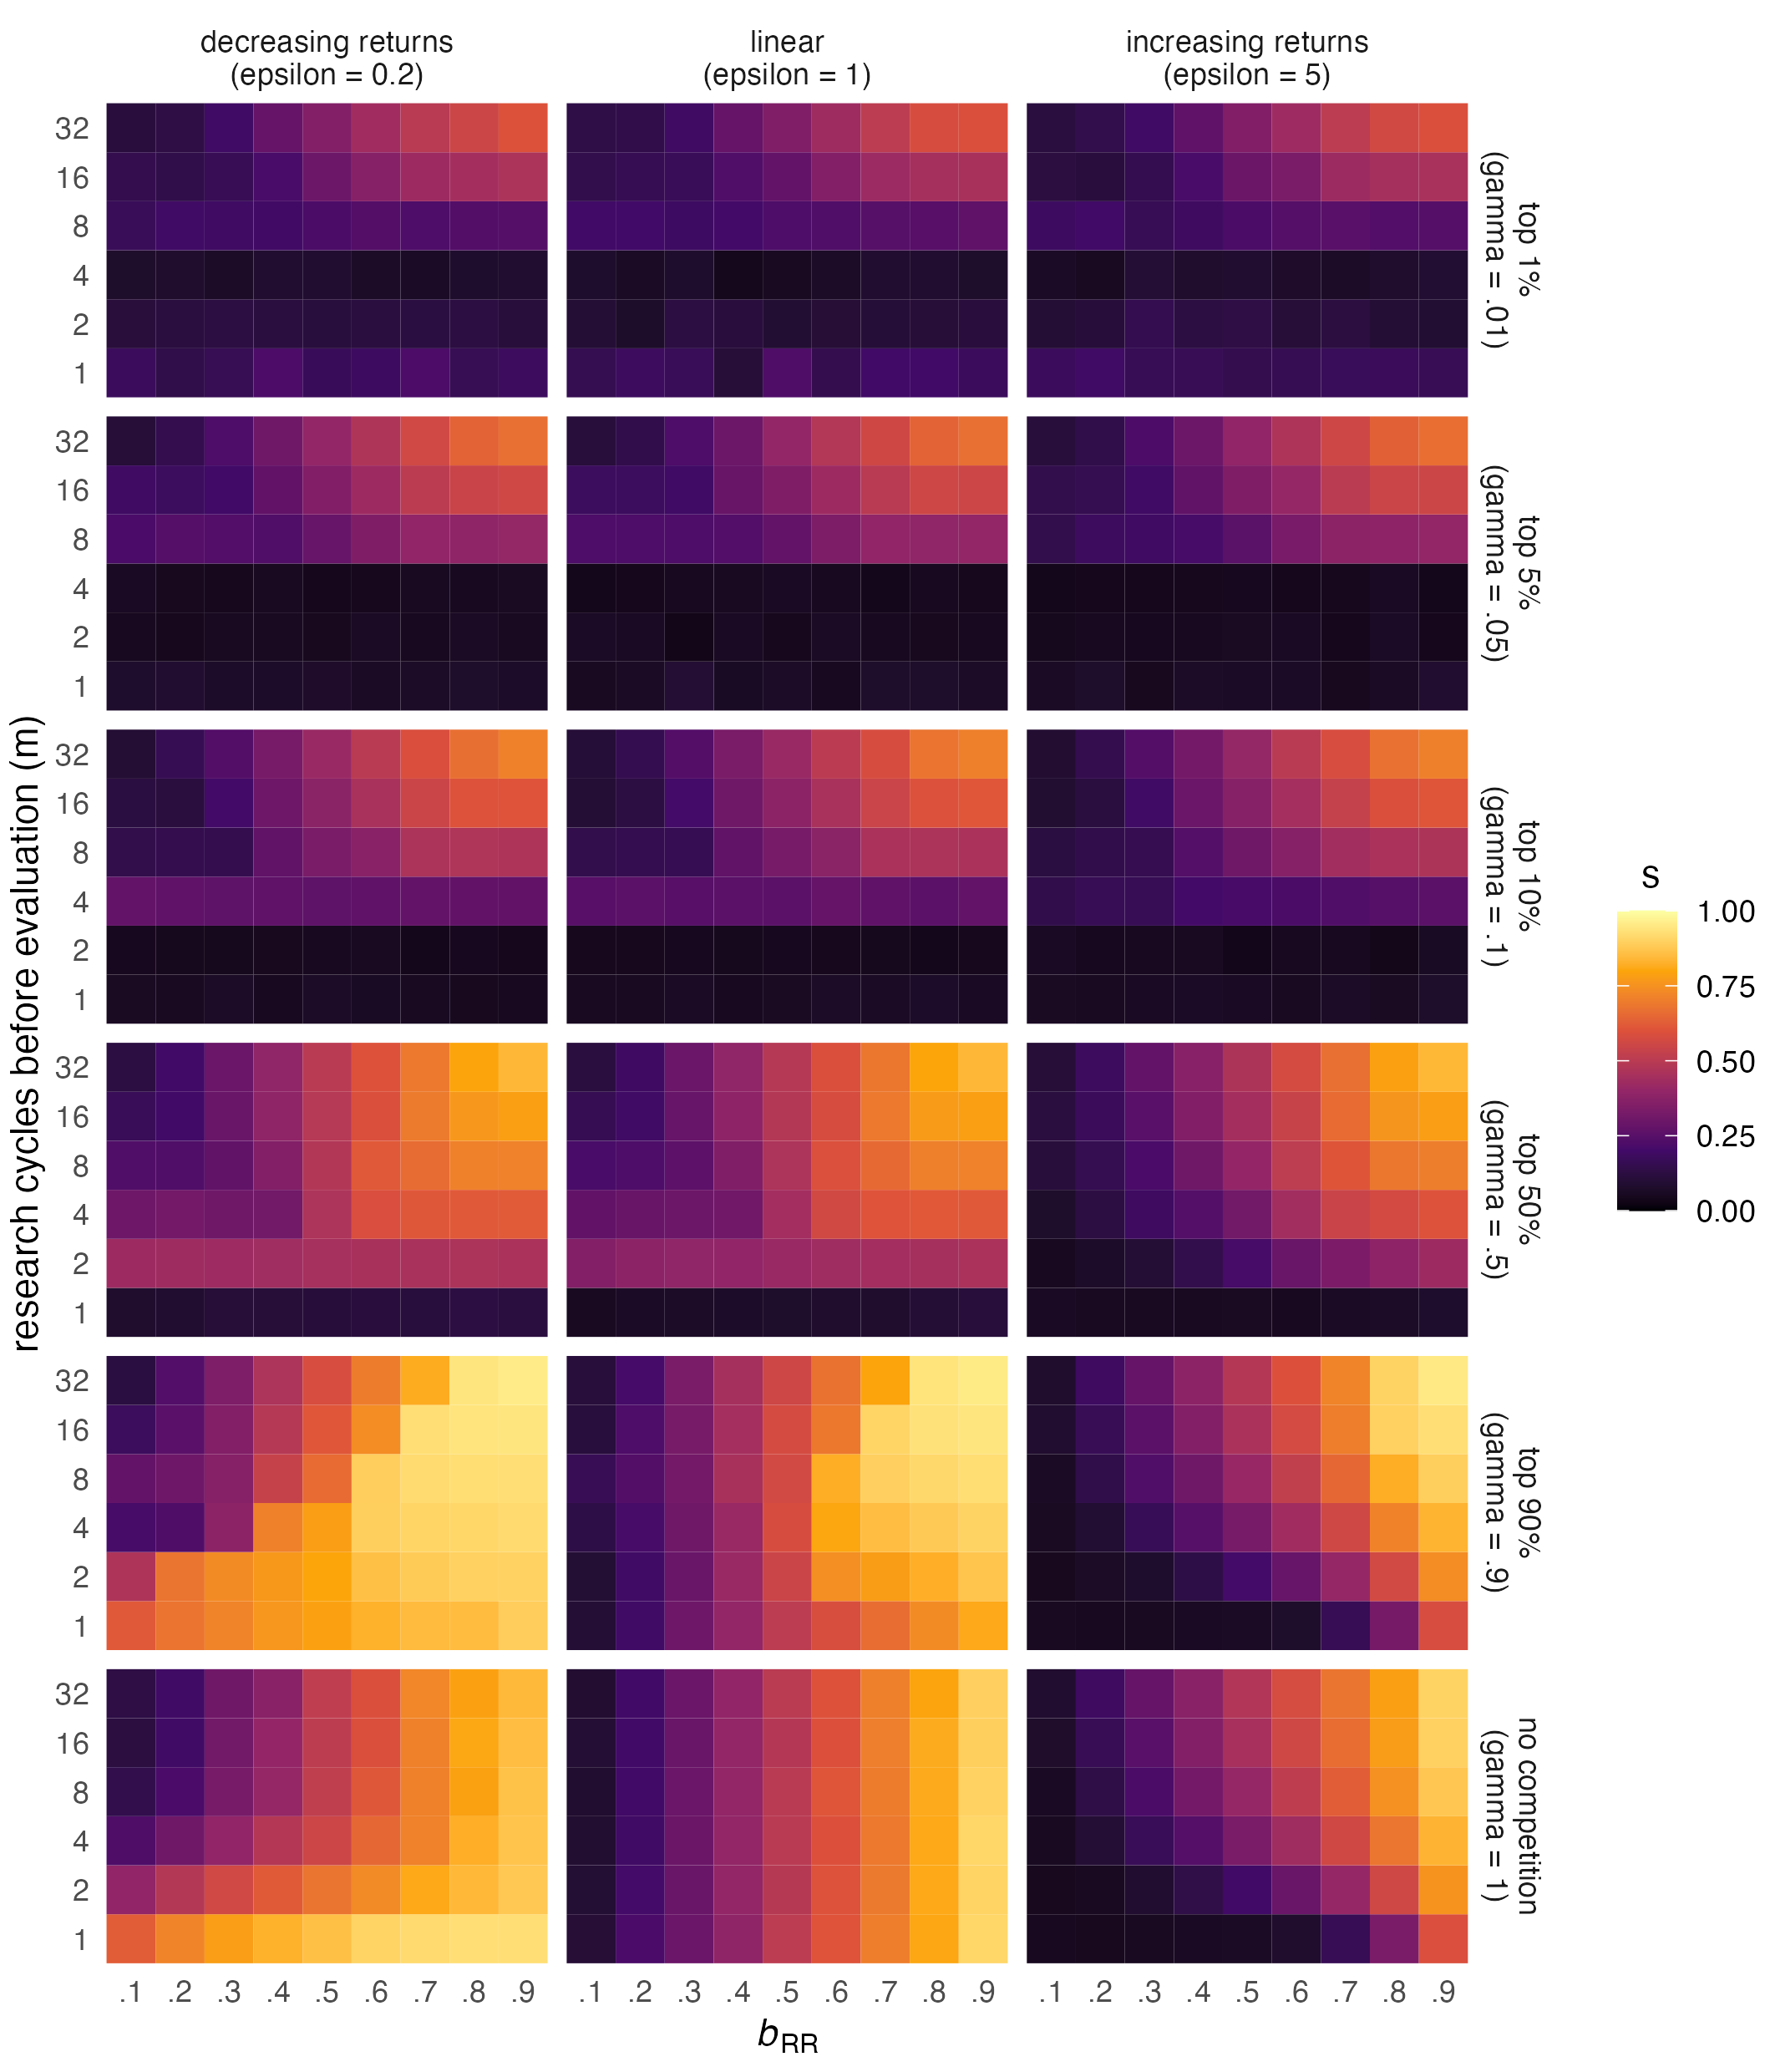
\includegraphics[width=1\linewidth]{plots/plot_gamma_evo_epsilon_inferno} \caption{Effect of competition on evolved publication strategies. Shown are median evolved publication strategies (\(s\)) after 250 generations in 50 runs (tile colour represents the median of 50 run medians) depending on the intensity of competition (\(\gamma\), y-axis), numbers of research cycles per generation (\(m\)), different values of \(b_{RR}\) (x-axis), and different fitness functions (characterised by exponent \(\epsilon\)) with no survival threshold (\(\delta = 0\)). To reproduce, researchers must accumulate a total payoff in the top \(\gamma\) proportion of the population.}\label{fig:competitionplot}
\end{figure}

\hypertarget{competition}{%
\subsection{Competition}\label{competition}}

Competition occurs whenever the demand for academic positions or grant funding exceeds the supply.
Figure \ref{fig:competitionplot} shows that competition generally leads to an aversion of Registered Reports, as can be seen by the darkening of the plots when moving up from the bottom row of panels.
The only exception to this rule is very low competition:
When the top 90\% are allowed to reproduce (and only the bottom 10\% are rejected, \(\gamma = .9\)), Registered Reports become more popular than they are in the absence of competition.
This effect is strongest for the concave fitness function (\(\epsilon = 0.2\)), where it holds for almost all values of \(b_{RR}\) at very low numbers of \(m\) and for high values of \(b_{RR}\) at high numbers of \(m\).
When the fitness function is linear or convex, Registered Reports are chosen more often only when both \(b_{RR}\) and \(m\) are high.
At higher levels of competition (\(\gamma > .5\)), the differences between the fitness functions disappear.
In all three cases, Registered Reports are essentially wiped out for low numbers of research cycles (\(m\)), and this effect increases with competition (the higher the competition, the higher \(m\) must be for Registered Reports to still be viable).
Intense competition also negatively affects Registered Reports at high numbers of \(m\), but here the general pattern of the baseline condition (a linear increase of Registered Reports popularity with \(b_{RR}\)) remains intact.

Looking at the first three rows of panels in Figure \ref{fig:competitionplot} (1\%, 5\%, and 10\% competition), the extreme effect of competition at low \(m\) appears to decrease slightly when competition is highest (\(\gamma = .01\)), indicated by the dark bar at the bottom of each panel becoming slightly lighter.
This paradoxial result is not due to Registered Reports being more lucrative in those conditions.
Rather, competition is so extreme that the natural selection in our model starts operating more on chance than on individuals' traits.
Essentially, only individuals with the maximum possible payoff (publishing only standard reports with positive results) are able to reproduce.
Most likely to receive this maximum payoff are individuals who investigate hypotheses with high prior probabilities.
In our model, this is not a trait that can be passed on, but determined by random chance.
Among individuals who experience this kind of luck, the variance of publication strategy \(s\) should be high:
A hypothesis with prior \(p = .95\) will be submitted as a standard report and likely yield a positive result (and thus the maximum payoff) regardless of whether the researcher's publication strategy is as low as \(s = .1\) or has high as \(s = .9\).
The higher average \(s\) at low \(m\) under extreme competition thus reflects relaxed selection pressure on \(s\).
This is also evident by the shades of the dark bar at the bottom of the panels for \(\gamma = .01\) (Fig. \ref{fig:competitionplot}), which fluctuate randomly for each level of \(m\) rather than showing a specific pattern.
A clearer illustration of the effect can be found in Figure XXX in the appendix, which shows large increases in the variance of evolved publication strategies in these conditions.
At higher \(m\), selection on \(s\) stays intact simply because much fewer individuals will be very lucky 4, 8, 16, or 32 times in a row than once or twice in a row, and publication strategy thus remains an important factor.

This effect of relaxed selection is not an arbitrary feature of our model, but commonly encountered in natural populations (Snyder, Ellner, \& Hooker, 2021).
In many species, luck can have an outsized impact on survival and reproduction, rendering the effects of individual traits relatively less important.
Luck does not eliminate natural selection\footnote{This is also apparent in Figure XXX (Appendix): Although the variance of evolved \(s\) increases dramatically with high competition, it never spans the entire range of \(s\).}, but it can significantly slow it.
XXX TRY LONGER SIM RUNS \& REPORT HERE XXX
The phenomenon is related to one form of survivorship bias:
Looking at `survivors' of a highly selective process, one may erroneously infer that specific observable traits or behaviours of such individuals were the cause of their success when those were actually merely coincidental.

In the academic world, researchers compete for tenured positions and grants.
The level of competition may vary between research areas, countries, institutions, grant programmes, and so on.
Our findings suggest that intense competition may be a significant threat for the viability of Registered Reports, regardless of career stage.
This effect is particularly extreme when very few research cycles can be completed before an evaluation event (e.g., in fields with low empirical pace, in labs with few resources, or on short-term contracts):
In such situations, publication strategies that involve any amount of Registered Reports are only viable when competition is so high that success requires extraordinary luck.
In contrast, very low but non-zero levels of competition increase the popularity of Registered Reports, especially when their value is high, when the fitness function is concave (e.g., in later career stages), and when researchers can complete many studies before being evaluated.

\hypertarget{discussion}{%
\section{Discussion}\label{discussion}}

In the artificial world of the model presented here, the standard publication route is a coin toss\(\,\)---\(\,\)the probability of obtaining a publishable result is 50\% on average\footnote{This is the case because we modelled the prior probability of tested hypotheses as being uniformly distributed between 0 and 1 and as being identical to the probability of obtaining a positive (i.e., publishable) result.}, translating to an expected payoff of 0.5 points per study.
If Registered Reports are a safe alternative to this gamble and guarantee publication in every case, one might think that payoff-maximising researchers would prefer them whenever they are worth more than
the expected payoff from standard reports and avoid them whenever they are worth less.
This intuition, however, rests on the assumption
that the career benefits researchers receive from publications are linear and involve no step changes.\footnote{Linearity is violated when the fitness function is concave or convex (\(\epsilon \neq |1|\)), but also in the presence of survival thresholds or competition, because these effectively introduce a step-change in the fitness function (low but non-zero payoffs yield zero career benefits).}
We argue that this assumption is violated in many, if not all, real-world situations.
Here, we investigated the impact of four factors that likely shape real-world situations:
convex vs concave fitness functions (additional publications yielding either increasing or decreasing returns, reflecting early vs later career stages), empirical pace (reflecting differences in speed and cost of data collection, available resources, or available time), survival thresholds (reflecting absolute publication targets researchers must meet in a given time), and competition for jobs or grants.
Our results show that in isolation or combined, many of these factors
would lead researchers with career-maximising strategies to avoid Registered Reports\(\,\)---\(\,\)even when Registered Reports are worth more than the expected payoff from standard reports.

To summarise the results, it is useful to take
the middle panel of Figure \ref{fig:mplot} (\(\epsilon = 1\)) as a baseline.
In this panel, publication payoffs translate into linear career benefits (the fitness curve is linear and there is no survival threshold and no competition), and the outcome is highly intuitive:
Researchers prefer Registered Reports whenever they are worth more than 0.5 points, and their preference is exactly proportional to \(b_{RR}\) and not affected by empirical pace.
Compared to this baseline, Registered Reports are \emph{less} popular when a) additional publications yield increasing returns (e.g., in early career) and empirical pace is low, b) when researchers face a survival threshold that cannot be met with Registered Reports alone, especially when publications yield decreasing returns once the threshold has been met (e.g., in advanced career stages) and empirical pace is low, and c) when there is substantial competition.
Competition has the most extreme effect and can cause a complete avoidance of Registered Reports when empirical pace is low.
Conversely, Registered Reports are \emph{more} popular than at baseline when a) additional publications yield decreasing returns and empirical pace is low, b) Registered Reports are worth just enough to reach a survival threshold and publications yield decreasing returns after the threshold is met, especially when empirical pace is low, and c) when there is very low but non-zero competition, especially when publications yield decreasing returns or empirical pace is high.

Looking at the interactions of the different factors, three observations stand out.
First, high empirical pace attenuates the effects of all other factors\(\,\)---\(\,\)at the highest pace we considered (32 research cycles before evaluation), outcomes are identical to baseline in almost all conditions.
The only exception to this rule is high competition, but although Registered Reports are relatively less attractive in this condition, the basic pattern is preserved and they remain viable when their value is high.
Second, the effect of survival thresholds strongly depends on the shape of the fitness function, suggesting that publication targets may have the strongest impact in advanced career stages.
Third, the opposite is true for high competition, which cancels out the effects of different fitness functions and thus appears to have virtually the same impact across career stages.

\begin{center}\rule{0.5\linewidth}{0.5pt}\end{center}

DRAFT COMPLETE UP UNTIL HERE

\hypertarget{implications}{%
\subsection{Implications}\label{implications}}

Our model predicts Registered Reports to be least popular when low empirical pace is combined with intense competition or with publication targets that cannot be met with Registered Reports alone.
Translated to real-world academia, this suggests that fields or labs in which productivity is limited by lacking resources or the cost or speed of data collection (e.g., research relying on expensive or rare equipment, research on populations that are difficult to access) deserve special attention.
Researchers in such situations may avoid the format when they must achieve publication targets that ask for a minimum number of publications in high-impact journals (e.g., as part of a tenure agreement), or when facing substantial competition for job positions or pressure to obtain competitive grants (e.g., if salary or research time depend on bringing in grants).
When competition is high, such researchers may favour standard reports even if Registered Reports are almost as valuable as the best possible outcome from a standard report.
Given that the last decades have seen vast increases in PhD students but relatively stable numbers of tenured positions in many countries (Cyranoski, Gilbert, Ledford, Nayar, \& Yahia, 2011), substantial competition may in fact be the default in many research fields, which could be one explanation for the currently low market share of Registered Reports.

\hypertarget{possible-interventions-to-increase-the-popularity-of-registered-reports}{%
\subsubsection{Possible interventions to increase the popularity of Registered Reports}\label{possible-interventions-to-increase-the-popularity-of-registered-reports}}

How can Registered Reports be made more attractive?
One answer, of course, is to change the just-mentioned situational factors that make Registered Reports unpopular.
However,
with the exception of tenure agreements and PhD regulations, these
factors are difficult to intervene on\(\,\)---\(\,\)competition and empirical pace cannot be changed easily, or at all.
A more feasible approach may be to change the payoff structure of Registered Reports relative to standard reports.
In the terms of our model, this could be achieved by increasing either the mean or the variance of the career-relevant payoffs that authors receive from a publication.
For simplicity, we treated payoffs as \emph{net} payoffs, meaning the difference between the benefits and costs of each publication route.
In reality,
the payoffs associated with Registered Reports can thus be raised by either increasing their benefits or lowering their costs (or both) relative to those of standard reports.
This implies three potential targets for intervention in total:
the benefits of Registered Reports, the costs of Registered Reports, and the variance of the net payoff of Registered Reports, each relative to standard reports.

\hypertarget{increasing-the-benefits-of-registered-reports}{%
\paragraph{Increasing the benefits of Registered Reports}\label{increasing-the-benefits-of-registered-reports}}

Our study was designed to investigate the consequences of the fact that whether and where a study is published is partly influenced by the study's results in standard reports, but not in Registered Reports.
We thus focus on the author benefits associated with the prestige and impact of the publishing journal (assuming that these parameters are both directly relevant for authors and causally influence citations, another relevant parameter, Traag, 2021).
In this regard, raising the benefits of Registered Reports could be achieved if more prestigious, high-impact journals offered the format.
High-impact journals may currently be particularly reluctant to offer
Registered Reports for fear of being forced to publish studies with uninteresting results, which might be cited less often.
Even when offering the format in principle, the same concern may lead such journals to be prohibitively selective during Stage-1 review and reject nearly all proposals.
Perhaps as the result of such a dynamic, the journal \emph{Nature} launched a Registered-Reports submission track in February 2023 (Nature, 2023), but appears to have published at most one Registered Report by August 2024.\footnote{We used the search function on \emph{Nature}'s website to search for the string `Registered Report' (entered without quotes) in research articles published since 22\textsuperscript{nd} February 2023 and then searched the full texts of the 72 search hits for the string `registered'. None of the articles was unambiguously marked as a Registered Report. Only one article (Aslett et al., 2024) contained the term `registered report' and was phrased in a way that may be consistent with the Registered Reports format.}
In practice, journals who are willing to participate in raising the value of Registered Reports should thus strive for designing an editorial process that, if ambitious, does not set unrealistic standards.

The value of Registered Reports can also be raised by those who ultimately provide the `career-relevant benefits' associated with a publication, namely faculty committees responsible for hiring and promotion decisions.
Placing a premium on Registered Reports in tenure agreements, promotion criteria, and hiring processes could increase the attractiveness of the format substantially.
This is in line with recent calls for greater emphasis on rigorous and transparent research methods in hiring, promotion, and tenure decisions (e.g., Moher et al., 2018), for example by including so-called `open-science statements' in job ads (Schönbrodt, 2016; Schönbrodt et al., 2018).
However, most such statements currently either do not define specific practices or mention only preregistration and not Registered Reports (Schönbrodt et al., 2018).
Explicitly highlighting Registered Reports in job ads and weighting them more heavily than standard reports in hiring, promotion, and tenure decisions could therefore be a promising strategy for increasing their popularity.

\hypertarget{decreasing-the-costs-of-registered-reports}{%
\paragraph{Decreasing the costs of Registered Reports}\label{decreasing-the-costs-of-registered-reports}}

Compared to standard reports, Registered Reports may be more costly for authors due to the additional stage of peer review
and stricter requirements for methodological rigour and sample size.
For example, Registered Reports (but not standard reports) in \emph{Nature Human Behaviour} currently must provide sampling plans aiming for at least \(95\%\) statistical power or a Bayes factor of 10 (Nature Human Behaviour, n.d.).
However, although it may be relatively easy to lower such standards,
doing so would also lower the value of Registered Reports to the scientific community (providing high-quality evidence) and thus partly defeat their purpose.
This problem illustrates that many of the additional costs associated with Registered Reports may be `good costs' that increase the quality of the resulting publications (see also Tiokhin, Yan, \& Morgan, 2021).
To preserve this quality, cost cutting may need to be confined to removing unnecessary inefficiencies, such as certain bureaucratic aspects of the submission or review process.

An alternative route to decreasing the relative costs of Registered Reports is to \emph{increase} the costs of standard reports.
Going back to the example above, a high-impact journal like \emph{Nature Human Behaviour} could reasonably demand the same level of methodological rigour
from standard reports as from Registered Reports.
This
would reduce the marginal advantage of standard reports over Registered Reports in terms of the investment required from authors (making Registered Reports relatively more attractive), while at the same time raising the quality of all studies published by the journal.

\hypertarget{increasing-payoff-variance}{%
\paragraph{Increasing payoff variance}\label{increasing-payoff-variance}}

\begin{itemize}
\tightlist
\item
  increase variance of pay-offs

  \begin{itemize}
  \tightlist
  \item
    PCI RR: increases potential maximum pay-offs --\textgreater get even better journals on board
  \end{itemize}
\end{itemize}

In Registered Reports,

The post-publication peer review platform \emph{Peer Community In} (PCI) recently launched a new model of Registered Reports (\emph{PCI Registered Reports}) in which authors are no longer tied to a specific journal.
\emph{PCI Registered Reports} offers authors the regular process of Stage-1 and Stage-2 review, but the end result of a successful submission is `only' a preprint with a so-called `recommendation' from \emph{PCI}.
Authors can subsequently publish their manuscript in one of several journals who partnered with \emph{PCI} and either rely on the \emph{PCI} review process alone or offer a streamlined review process for \emph{PCI}-recommended preprints.
Alternatively, authors are free to submit to any other journal as if their manuscript were a standard report.
This innovation gives Registered-Reports authors significantly more freedom to capitalise on the results of their study because a submission to PCI Registered Reports does not preclude the chance of a high-impact publication.
PCI Registered Reports thus constitute a significant change to the relative incentives and risk structure of Registered Reports compared to standard reports that merits a closer investigation in the future.

\hypertarget{general-implications-for-risk-taking-in-academic-research}{%
\subsubsection{General implications for risk-taking in academic research}\label{general-implications-for-risk-taking-in-academic-research}}

\begin{itemize}
\tightlist
\item
  Implications for risk taking more generally

  \begin{itemize}
  \tightlist
  \item
    apply findings to different situations
  \item
    for example, implications for funding lotteries?
  \end{itemize}
\end{itemize}

The core of our model is the choice between a high-risk option and a low-risk option, with `risk' meaning unpredictable variability in outcomes.
We assume that the standard publication route always has greater risk than conducting a Registered Report.

Our model also predicts that low but non-zero competition \emph{increases} the popularity of Registered Reports relative to baseline.
This result is interesting in light of proposals for replacing traditional grant funding competitions with modified lotteries, in which grants are raffled between applicants whose proposals clear a certain quality threshold (Fang \& Casadevall, 2016; Heyard, Ott, Salanti, \& Egger, 2022; Smaldino, Turner, \& Contreras Kallens, 2019).
Modified lotteries would represent low but non-zero competition if the quality threshold was set very low (e.g., excluding only the bottom 10\% of proposals).
Whether such low-threshold lotteries would have a measurable effect on the popularity of Registered Reports is questionable because applicants' publication records are usually not a primary criterion for funding decisions (although they may have a sizeable influence on reviews, Simsek, de Vaan, \& van de Rijt, 2024).
However, a more general interpretation of our results is

In contrast, researchers in fields or labs with very high empirical pace (e.g., research areas relying on online surveys) should remain relatively indifferent to Registered Reports, preferring them when they are worth more than the expected payoff from the standard publication route and avoiding them when they are worth less than that.
The only exception to this are situations with intense competition, which drives such researchers to avoid Registered Reports unless they are very valuable (e.g., when Registered Reports can be conducted at the best journal that researchers think would publish their study as a standard report).

High levels competition may in fact be the default in many disciplines and countries, as the last decades have seen vast increases in PhD graduates but relatively stable numbers of tenured positions (Cyranoski et al., 2011).
Given that the last decades have seen vast increases in PhD students but relatively stable numbers of tenured positions in many countries (Cyranoski et al., 2011), substantial competition may in fact be the default in many research fields.

The simulation results we presented show clearly that the lower risk associated with Registered Reports does not automatically make them more attractive.
Instead, we find many situations in which career-maximising researchers may favour the standard publication route or even avoid Registered Reports entirely.
Most prominently, our model predicts such complete avoidance when competition is high and empirical pace\(\,\)---\(\,\)the number of studies researchers can complete before evaluation\(\,\)---\(\,\)is low.
In this constellation, Registered Reports are not sustainable even if their value is almost as high as the maximum payoff that authors can achieve through the standard route.
Substantial competition may in fact be the default in many disciplines and countries, as the last decades have seen vast increases in PhD graduates but relatively stable numbers of tenured positions (Cyranoski et al., 2011).
This factor might thus be part of the explanation for the very low market share of Registered Reports.
Two interesting question to study empirically would be 1) whether attitudes towards the format vary between researchers who experience different levels of competition (e.g., between regions or research fields) and 2) whether this effect, if present, is stronger in fields or labs where productivity is limited by slow data collection or lacking resources (low empirical pace).

Another, less intuitive prediction of the model is that Registered Reports should be avoided by early-career researchers and preferred by more senior researchers, again particularly when empirical pace is low.
This is based on the assumption that additional publications provide increasing returns for a junior researcher's career but decreasing returns for a senior researcher's career.

Although Registered Reports have existed for over ten years at this point, surprisingly little is known about who uses the format and for what

The most fundamental assumption of our model is that the career-relevant benefit authors receive from trying to publish a study varies less in Registered Reports than in standard reports.
When this is true, and when the benefit associated with a Registered Report is lower than the maximum benefit authors could receive from a standard report, Registered Reports will often be an unattractive choice.

have lower unpredictable outcome variability (risk) than the standard publication route

The summary above highlights several situations in which a low-risk publication option may not be in researchers' interest.

The model we presented focuses on the difference in risk\(\,\)---\(\,\)unpredictable outcome variance\(\,\)---\(\,\)between Registered Reports and the standard publication route.
The goal of this study was to achieve a better understanding of the consequences of this difference and to identify situations in which Registered Reports may remain unattractive without further intervention, or be used in highly selective ways.

\texttt{To\ do:}

\begin{itemize}
\tightlist
\item
  Implications of results

  \begin{itemize}
  \item
    high competition may be the default: jobs, grants
  \item
    job selection not only on publication record. Beyond a certain threshold, more pubs may not matter much --\textgreater{} this basically means the fitness curve is concave
  \item
    \emph{low} competition may actually be good for grants: supports proposals for lotteries (after sifting out low-quality proposals) but not egalitarian funding distribution
  \item
    ECRs predicted to avoid RRs unless empirical pace is high or they want to leave academia --\textgreater{} conflicts with empirical finding suggesting that RRs are more likely to have junior first authors
  \item
    Tian, Su, \& Ru (2016): there are cases of high survival thresholds
  \item
    potential implications for meta-science
  \item
    potential implications for policy
  \end{itemize}
\end{itemize}

\hypertarget{limitations-and-future-directions}{%
\subsection{Limitations and future directions}\label{limitations-and-future-directions}}

\begin{itemize}
\tightlist
\item
  General ``limitation'' of formal modeling

  \begin{itemize}
  \tightlist
  \item
    Narrow focus, ignores many important factors (by design)
  \end{itemize}
\end{itemize}

By design, our model is based on assumptions that simplify and exaggerate some aspects of real-world academia and ignore many others.
First, we use an extreme, cartoonish concept of publication bias and its relation to the prior probability of tested hypotheses:
All positive results are published, all negative results remain unpublished, and results are determined only by the prior probability of hypotheses.

\begin{itemize}
\tightlist
\item
  Concept of publication bias as filtering positive results of hypothesis tests (and the respective connection to hypothesis priors such that high priors --\textgreater{} better) is cartoonish and not entirely accurate for the simple reason that positive results of trivial (or otherwise boring) hypotheses are usually not highly valued (also, this approach only focuses on hypothesis testing, which is widely used in psychology but by far not the only means of doing science).
  A more valid solution may be the concept of publication bias as favouring belief-shifting results presented by Gross \& Bergstrom (2021).
  Adapting the model presented here to capture this concept of bias could be an interesting future direction.
  However, the present version of the model also allows a conservative interpretation in which the prior probability of hypotheses simply reflects authors' predictions of the eventual publication value of different research questions.
  This interpretation is still concordant with Registered Reports and standard reports differing in risk, because the publication value of standard reports certainly depends more strongly on the study results than the publication value of Registered Reports (even if not in the simplistic sense of positive hypothesis tests having higher value).
\end{itemize}

The purpose of this simulation study was to understand the effects of a small set of factors on author incentives for Registered Reports.
Although this narrow focus ignores many other factors that play a role in real-world academia, the simulation results can be used to identify targets for further investigation.
Specifically, our model predicts several situations in which researchers might avoid Registered Reports entirely.

be used as a starting point for further investigation.
provide a general expectation about the
we can use the results
the simulation results can help develop general expectations about the studied variables (making `all else being equal' predictions)
it allows us to infer general patterns
likely influence the adoption of Registered Reports in real-world academia,

Our model isolates a small set of factors
The purpose of this narrow focus
This narrow focus allowed us to isolate the
The simulation results thus cannot and should not be mapped directly onto specific real-world situations.
However, the results can be used to identify
The purpose of this study was instead to help form an intuition and develop general expectations about the effects of specific factors in isolation (i.e., all else being equal).

In addition, situations
In addition to suggesting general trends, our results point to a number of situations in which these factors appear to drastically reduce the attractiveness of Registered Reports.
For meta-scientists and for advocates of the format, these situations are targets for further investigation.

\begin{itemize}
\tightlist
\item
  cartoonish concept of publication bias

  \begin{itemize}
  \tightlist
  \item
    simplest fix: make it noisier/probabilistic --\textgreater{} likely result: more noisy in the outcome
  \item
    more realistic: model additional dimensions of papers
  \item
    simplification probably fine for the purposes
  \end{itemize}
\item
  assignment of prior probability

  \begin{itemize}
  \tightlist
  \item
    prior probably not uniform across 0 and 1

    \begin{itemize}
    \tightlist
    \item
      many more wrong? but many also trivially true?
    \item
      can try different distributions
    \end{itemize}
  \item
    in all cycles randomly drawn hypothesis -- not realistic, researchers pick hypotheses

    \begin{itemize}
    \tightlist
    \item
      ability-based risk taking
    \item
      (Optional/low priority: perfect knowledge about prior; how accurate is knowledge in practice? Interindividual difference in knowledge about prior?)
    \end{itemize}
  \end{itemize}
\end{itemize}

\hypertarget{ability-based-risk-taking}{%
\paragraph{Ability-based risk taking}\label{ability-based-risk-taking}}

The model presented in this chapter only considers the effects of situational factors on individuals' risk sensitivity.
However, risk sensitivity can also be influenced by individual differences, such that individuals with traits or abilities that increase their expected payoff from a risky option (e.g., traits that increase their winning chances or the payoff when winning or that buffer the impact of losses) should be more risk-prone (Barclay, Mishra, \& Sparks, 2018).
Such factors may be important to consider in the context of research and publication practices.
For example, researchers who are better at choosing research questions that are likely to result in high-impact publications (e.g., through talent or experience) may find Registered Reports less attractive.
As a more nefarious version of this idea, Registered Reports may be relatively unpopular among researchers who are more inclined to using questionable research practices (or even fraud) to obtain publishable or impactful results.

\begin{itemize}
\tightlist
\item
  ignores time as a factor

  \begin{itemize}
  \tightlist
  \item
    mean and/or variance of time to publication may differ between RRs and SRs, and people may discount delays
  \end{itemize}
\end{itemize}

\begin{itemize}
\item
  model assumes researchers working alone

  \begin{itemize}
  \tightlist
  \item
    senior researchers also have to take needs of ECRs into account etc.
  \item
    empirical pace compensated for by increased number of co-authors? -\textgreater{} future bibliometric analyses
  \end{itemize}
\item
  Narrow focus on one specific (and highly stylised) difference between Registered Reports and standard reports; there are many others. Model ignores a myriad other factors that influences who chooses Registered Reports for which studies when
\item
  Fitness concept: one caveat is that
\item
  RRs may actually \emph{slow} the empirical pace, introducing an interaction that our model doesn't take into account
\end{itemize}

\hypertarget{conclusion}{%
\subsection{Conclusion}\label{conclusion}}

Around 600,000 journal articles per year are published in psychology alone.\footnote{Estimate was obtained via \url{https://lens.org} by applying the filters \texttt{Year\ Published\ =\ 2020-\/-2023}, \texttt{Publication\ Type\ =\ journal\ article}, and \texttt{Field\ of\ Study\ =\ Psychology}, and dividing the 2,448,670 resulting hits by 4.}
Compared to this, the 591 Registered Reports published by 2021 (Chambers \& Tzavella, 2022) are a tiny number\(\,\)---\(\,\)even assuming that all of them were psychological studies and published in just one year, they would represent less than \(0.10\%\) of the literature.
This figure is much lower than the estimated prevalence of preregistration in the psychology literature (\(7\%\) 2002, \(95\%\) CI = {[}\(2.5\%\)--\(12\%\){]}, Hardwicke et al., 2024), a reform that was introduced around the same time with similar goals (reducing bias in published results).
The difference in adoption rates could reflect that Registered Reports require a more profound change to researchers' habitual workflow, are more costly in other ways (e.g., require larger samples), are not available at all journals (although more than 300 journals offer them at this point) or simply are less well known.
Nonetheless, one might expect the format to spread more quickly if it offered substantial advantages for researchers' careers.

\begin{itemize}
\tightlist
\item
  add here that this might be explained by high competition being the default
  High levels competition may in fact be the default in many scientific disciplines and countries, as the last decades have seen vast increases in PhD graduates but relatively stable numbers of tenured positions (Cyranoski et al., 2011).
\end{itemize}

\hypertarget{disclosures}{%
\subsection{Disclosures}\label{disclosures}}

\hypertarget{data-materials-and-online-resources}{%
\subsubsection{Data, materials, and online resources}\label{data-materials-and-online-resources}}

This manuscript was created using RStudio (1.2.5019, RStudio Team, 2019) and R (Version 4.2.1; R Core Team, 2019) and the R-packages \emph{bookdown} (Version 0.34; Xie, 2016), \emph{ggplot2} (Version 3.5.0; Wickham, 2016), \emph{here} (Version 1.0.1; K. Müller, 2017), \emph{knitr} (Version 1.46; Xie, 2015), \emph{papaja} (Version 0.1.1.9001; Aust \& Barth, 2018), \emph{rmarkdown} (Version 2.26; Xie, Allaire, \& Grolemund, 2018), \emph{stringr} (Version 1.5.1; Wickham, 2023), and \emph{tinylabels} (Version 0.2.3; Barth, 2022).

\hypertarget{references}{%
\section{References}\label{references}}

\setlength{\parindent}{-0.2in}
\setlength{\leftskip}{0.2in}


\hypertarget{refs}{}
\begin{CSLReferences}{1}{0}
\leavevmode\vadjust pre{\hypertarget{ref-Agnoli2017}{}}%
Agnoli, F., Wicherts, J. M., Veldkamp, C. L. S., Albiero, P., \& Cubelli, R. (2017). Questionable research practices among italian research psychologists. \emph{PLOS ONE}, \emph{12}(3), e0172792. \url{https://doi.org/10.1371/journal.pone.0172792}

\leavevmode\vadjust pre{\hypertarget{ref-Allen2019}{}}%
Allen, C., \& Mehler, D. M. A. (2019). Open science challenges, benefits and tips in early career and beyond. \emph{PLOS Biology}, \emph{17}(5), e3000246. \url{https://doi.org/10.1371/journal.pbio.3000246}

\leavevmode\vadjust pre{\hypertarget{ref-Aslett2024}{}}%
Aslett, K., Sanderson, Z., Godel, W., Persily, N., Nagler, J., \& Tucker, J. A. (2024). Online searches to evaluate misinformation can increase its perceived veracity. \emph{Nature}, \emph{625}(7995), 548--556. \url{https://doi.org/10.1038/s41586-023-06883-y}

\leavevmode\vadjust pre{\hypertarget{ref-Atkinson1982}{}}%
Atkinson, D. R., Furlong, M. J., \& Wampold, B. E. (1982). Statistical significance, reviewer evaluations, and the scientific process: {Is} there a (statistically) significant relationship? \emph{Journal of Counseling Psychology}, \emph{29}(2), 189--194. \url{https://doi.org/10.1037/0022-0167.29.2.189}

\leavevmode\vadjust pre{\hypertarget{ref-R-papaja}{}}%
Aust, F., \& Barth, M. (2018). \emph{{papaja}: {Create APA} manuscripts with {R Markdown}}.

\leavevmode\vadjust pre{\hypertarget{ref-Barclay2018}{}}%
Barclay, P., Mishra, S., \& Sparks, A. M. (2018). State-dependent risk-taking. \emph{Proceedings of the Royal Society B: Biological Sciences}, \emph{285}(1881), 20180180. \url{https://doi.org/10.1098/rspb.2018.0180}

\leavevmode\vadjust pre{\hypertarget{ref-R-tinylabels}{}}%
Barth, M. (2022). \emph{{tinylabels}: Lightweight variable labels}. Retrieved from \url{https://cran.r-project.org/package=tinylabels}

\leavevmode\vadjust pre{\hypertarget{ref-Chalmers2009}{}}%
Chalmers, I., \& Glasziou, P. (2009). Avoidable waste in the production and reporting of research evidence. \emph{The Lancet}, \emph{374}(9683), 86--89. \url{https://doi.org/10.1016/S0140-6736(09)60329-9}

\leavevmode\vadjust pre{\hypertarget{ref-Chambers2013}{}}%
Chambers, C. D. (2013). Registered reports: {A} new publishing initiative at {Cortex}. \emph{Cortex}, \emph{49}, 606--610. \url{https://doi.org/10.1016/j.cortex.2012.12.016}

\leavevmode\vadjust pre{\hypertarget{ref-Chambers2015}{}}%
Chambers, C. D., Dienes, Z., McIntosh, R. D., Rotshtein, P., \& Willmes, K. (2015). Registered {Reports}: {Realigning} incentives in scientific publishing. \emph{Cortex}, \emph{66}, 1--2. \url{https://doi.org/10.1016/j.cortex.2015.03.022}

\leavevmode\vadjust pre{\hypertarget{ref-Chambers2022}{}}%
Chambers, C. D., \& Tzavella, L. (2022). The past, present and future of {Registered Reports}. \emph{Nature Human Behaviour}, \emph{6}(1), 29--42. \url{https://doi.org/10.1038/s41562-021-01193-7}

\leavevmode\vadjust pre{\hypertarget{ref-Cubitt2001}{}}%
Cubitt, R. P., Starmer, C., \& Sugden, R. (2001). Discovered preferences and the experimental evidence of violations of expected utility theory. \emph{Journal of Economic Methodology}, \emph{8}(3), 385--414. \url{https://doi.org/10.1080/13501780110103748}

\leavevmode\vadjust pre{\hypertarget{ref-Cyranoski2011}{}}%
Cyranoski, D., Gilbert, N., Ledford, H., Nayar, A., \& Yahia, M. (2011). Education: {The PhD} factory. \emph{Nature}, \emph{472}(7343), 276--279. \url{https://doi.org/10.1038/472276a}

\leavevmode\vadjust pre{\hypertarget{ref-deVries2018}{}}%
de Vries, Y. A., Roest, A. M., Jonge, P. de, Cuijpers, P., Munafò, M. R., \& Bastiaansen, J. A. (2018). The cumulative effect of reporting and citation biases on the apparent efficacy of treatments: The case of depression. \emph{Psychological Medicine}, \emph{48}(15), 2453--2455. \url{https://doi.org/10.1017/S0033291718001873}

\leavevmode\vadjust pre{\hypertarget{ref-Dickersin1993}{}}%
Dickersin, K., \& Min, Y. I. (1993). Publication bias: The problem that won't go away. \emph{Annals of the New York Academy of Sciences}, \emph{703}, 135-146; discussion 146-148. \url{https://doi.org/10.1111/j.1749-6632.1993.tb26343.x}

\leavevmode\vadjust pre{\hypertarget{ref-Driessen2015}{}}%
Driessen, E., Hollon, S. D., Bockting, C. L. H., Cuijpers, P., \& Turner, E. H. (2015). Does {Publication Bias Inflate} the {Apparent Efficacy} of {Psychological Treatment} for {Major Depressive Disorder}? {A Systematic Review} and {Meta-Analysis} of {US National Institutes} of {Health-Funded Trials}. \emph{PLOS ONE}, \emph{10}(9), e0137864. \url{https://doi.org/10.1371/journal.pone.0137864}

\leavevmode\vadjust pre{\hypertarget{ref-Ensinck2023}{}}%
Ensinck, E., \& Lakens, D. (2023). \emph{An {Inception Cohort Study Quantifying How Many Registered Studies} are {Published}}. PsyArXiv. \url{https://doi.org/10.31234/osf.io/5hkjz}

\leavevmode\vadjust pre{\hypertarget{ref-Fang2016}{}}%
Fang, F. C., \& Casadevall, A. (2016). Research {Funding}: The {Case} for a {Modified Lottery}. \emph{mBio}. \url{https://doi.org/10.1128/mbio.00422-16}

\leavevmode\vadjust pre{\hypertarget{ref-Ferguson2012}{}}%
Ferguson, C. J., \& Heene, M. (2012). A {Vast Graveyard} of {Undead Theories}: {Publication Bias} and {Psychological Science}'s {Aversion} to the {Null}. \emph{Perspectives on Psychological Science}, \emph{7}(6), 555--561. \url{https://doi.org/10.1177/1745691612459059}

\leavevmode\vadjust pre{\hypertarget{ref-Fiedler2016}{}}%
Fiedler, K., \& Schwarz, N. (2016). Questionable {Research Practices Revisited}. \emph{Social Psychological and Personality Science}, \emph{7}(1), 45--52. \url{https://doi.org/10.1177/1948550615612150}

\leavevmode\vadjust pre{\hypertarget{ref-Franco2014}{}}%
Franco, A., Malhotra, N., \& Simonovits, G. (2014). Publication bias in the social sciences: {Unlocking} the file drawer. \emph{Science}, \emph{345}(6203), 1502--1505. \url{https://doi.org/10.1126/science.1255484}

\leavevmode\vadjust pre{\hypertarget{ref-Franco2016}{}}%
Franco, A., Malhotra, N., \& Simonovits, G. (2016). Underreporting in {Psychology Experiments}: {Evidence From} a {Study Registry}. \emph{Social Psychological and Personality Science}, \emph{7}(1), 8--12. \url{https://doi.org/10.1177/1948550615598377}

\leavevmode\vadjust pre{\hypertarget{ref-Fraser2018}{}}%
Fraser, H., Parker, T., Nakagawa, S., Barnett, A., \& Fidler, F. (2018). Questionable research practices in ecology and evolution. \emph{PLOS ONE}, \emph{13}(7), e0200303. \url{https://doi.org/10.1371/journal.pone.0200303}

\leavevmode\vadjust pre{\hypertarget{ref-Gerber2001}{}}%
Gerber, A. S., Green, D. P., \& Nickerson, D. (2001). Testing for {Publication Bias} in {Political Science}. \emph{Political Analysis}, \emph{9}(4), 385--392. \url{https://doi.org/10.1093/oxfordjournals.pan.a004877}

\leavevmode\vadjust pre{\hypertarget{ref-Gopalakrishna2022}{}}%
Gopalakrishna, G., Wicherts, J. M., Vink, G., Stoop, I., Akker, O. R. van den, Riet, G. ter, \& Bouter, L. M. (2022). \emph{Prevalence of responsible research practices among academics in {The Netherlands}}. \emph{11}(471). \url{https://doi.org/10.12688/f1000research.110664.2}

\leavevmode\vadjust pre{\hypertarget{ref-Greenwald1975}{}}%
Greenwald, A. G. (1975). Consequences of {Prejudice Against} the {Null Hypothesis}. \emph{Psychological Bulletin}, \emph{82}(1), 1--20.

\leavevmode\vadjust pre{\hypertarget{ref-Gross2021}{}}%
Gross, K., \& Bergstrom, C. T. (2021). Why ex post peer review encourages high-risk research while ex ante review discourages it. \emph{Proceedings of the National Academy of Sciences}, \emph{118}(51). \url{https://doi.org/10.1073/pnas.2111615118}

\leavevmode\vadjust pre{\hypertarget{ref-Haaland2019}{}}%
Haaland, T. R., Wright, J., \& Ratikainen, I. I. (2019). Bet-hedging across generations can affect the evolution of variance-sensitive strategies within generations. \emph{Proceedings of the Royal Society B}. \url{https://doi.org/10.1098/rspb.2019.2070}

\leavevmode\vadjust pre{\hypertarget{ref-Hardwicke2024}{}}%
Hardwicke, T. E., Thibault, R. T., Clarke, B., Moodie, N., Crüwell, S., Schiavone, S. R., \ldots{} Vazire, S. (2024). \emph{Prevalence of transparent research practices in psychology: {A} cross-sectional study of empirical articles published in 2022}. OSF. \url{https://doi.org/10.31234/osf.io/t2zs9}

\leavevmode\vadjust pre{\hypertarget{ref-Heyard2022}{}}%
Heyard, R., Ott, M., Salanti, G., \& Egger, M. (2022). Rethinking the {Funding Line} at the {Swiss National Science Foundation}: {Bayesian Ranking} and {Lottery}. \emph{Statistics and Public Policy}, \emph{9}(1), 110--121. \url{https://doi.org/10.1080/2330443X.2022.2086190}

\leavevmode\vadjust pre{\hypertarget{ref-Higginson2016}{}}%
Higginson, A. D., \& Munafò, M. R. (2016). Current {Incentives} for {Scientists Lead} to {Underpowered Studies} with {Erroneous Conclusions}. \emph{PLOS Biology}, \emph{14}(11), e2000995. \url{https://doi.org/10.1371/journal.pbio.2000995}

\leavevmode\vadjust pre{\hypertarget{ref-Hurly2003}{}}%
Hurly, A. T. (2003). The twin threshold model: Risk-intermediate foraging by rufous hummingbirds, {Selasphorus} rufus. \emph{Animal Behaviour}, \emph{66}(4), 751--761. \url{https://doi.org/10.1006/anbe.2003.2278}

\leavevmode\vadjust pre{\hypertarget{ref-John2012}{}}%
John, L. K., Loewenstein, G., \& Prelec, D. (2012). Measuring the {Prevalence} of {Questionable Research Practices With Incentives} for {Truth Telling}. \emph{Psychological Science}, \emph{23}(5), 524--532. \url{https://doi.org/10.1177/0956797611430953}

\leavevmode\vadjust pre{\hypertarget{ref-Kacelnik1996}{}}%
Kacelnik, A., \& Bateson, M. (1996). Risky {Theories}---{The Effects} of {Variance} on {Foraging Decisions}. \emph{Integrative and Comparative Biology}, \emph{36}(4), 402--434. \url{https://doi.org/10.1093/icb/36.4.402}

\leavevmode\vadjust pre{\hypertarget{ref-Kacelnik1997}{}}%
Kacelnik, A., \& Bateson, M. (1997). Risk-sensitivity: Crossroads for theories of decision-making. \emph{Trends in Cognitive Sciences}, \emph{1}(8), 304--309. \url{https://doi.org/10.1016/s1364-6613(97)01093-0}

\leavevmode\vadjust pre{\hypertarget{ref-Kepes2022}{}}%
Kepes, S., Keener, S. K., McDaniel, M. A., \& Hartman, N. S. (2022). Questionable research practices among researchers in the most research-productive management programs. \emph{Journal of Organizational Behavior}, \emph{43}(7), 1190--1208. \url{https://doi.org/10.1002/job.2623}

\leavevmode\vadjust pre{\hypertarget{ref-Kerr1998}{}}%
Kerr, N. L. (1998). {HARKing}: {Hypothesizing} after the results are known. \emph{Personality and Social Psychology Review}, \emph{2}(3), 196--217. \url{https://doi.org/10.1207/s15327957pspr0203_4}

\leavevmode\vadjust pre{\hypertarget{ref-Liner2009}{}}%
Liner, G. H., \& Sewell, E. (2009). Research requirements for promotion and tenure at {PhD} granting departments of economics. \emph{Applied Economics Letters}. \url{https://doi.org/10.1080/13504850701221998}

\leavevmode\vadjust pre{\hypertarget{ref-Mahoney1977}{}}%
Mahoney, M. J. (1977). Publication {Prejudices}: {An Experimental Study} of {Confirmatory Bias} in the {Peer Review System}. \emph{Cognitive Therapy and Research}, \emph{1}(2), 161--175. \url{https://doi.org/10.1007/BF01173636}

\leavevmode\vadjust pre{\hypertarget{ref-Makel2021}{}}%
Makel, M. C., Hodges, J., Cook, B. G., \& Plucker, J. A. (2021). Both {Questionable} and {Open Research Practices Are Prevalent} in {Education Research}: \emph{Educational Researcher}. \url{https://doi.org/10.3102/0013189X211001356}

\leavevmode\vadjust pre{\hypertarget{ref-Miller2011a}{}}%
Miller, A. N., Taylor, S. G., \& Bedeian, A. G. (2011). Publish or perish: Academic life as management faculty live it. \emph{Career Development International}, \emph{16}(5), 422--445. \url{https://doi.org/10.1108/13620431111167751}

\leavevmode\vadjust pre{\hypertarget{ref-Mishra2014}{}}%
Mishra, S. (2014). Decision-{Making Under Risk}: {Integrating Perspectives From Biology}, {Economics}, and {Psychology}. \emph{Personality and Social Psychology Review}, \emph{18}(3), 280--307. \url{https://doi.org/10.1177/1088868314530517}

\leavevmode\vadjust pre{\hypertarget{ref-Moher2018}{}}%
Moher, D., Naudet, F., Cristea, I. A., Miedema, F., Ioannidis, J. P. A., \& Goodman, S. N. (2018). Assessing scientists for hiring, promotion, and tenure. \emph{PLOS Biology}, \emph{16}(3), e2004089. \url{https://doi.org/10.1371/journal.pbio.2004089}

\leavevmode\vadjust pre{\hypertarget{ref-R-here}{}}%
Müller, K. (2017). \emph{Here: {A} simpler way to find your files}.

\leavevmode\vadjust pre{\hypertarget{ref-Muller2014}{}}%
Müller, R. (2014). Postdoctoral {Life Scientists} and {Supervision Work} in the {Contemporary University}: {A Case Study} of {Changes} in the {Cultural Norms} of {Science}. \emph{Minerva}, \emph{52}(3), 329--349. \url{https://doi.org/10.1007/s11024-014-9257-y}

\leavevmode\vadjust pre{\hypertarget{ref-Muller2017}{}}%
Müller, R., \& de Rijcke, S. (2017). Thinking with indicators. {Exploring} the epistemic impacts of academic performance indicators in the life sciences. \emph{Research Evaluation}, \emph{26}(3), 157--168. \url{https://doi.org/10.1093/reseval/rvx023}

\leavevmode\vadjust pre{\hypertarget{ref-Nature2023}{}}%
Nature. (2023). Nature welcomes {Registered Reports}. \emph{Nature}, \emph{614}(7949), 594--594. \url{https://doi.org/10.1038/d41586-023-00506-2}

\leavevmode\vadjust pre{\hypertarget{ref-NatureHumanBehaviour}{}}%
Nature Human Behaviour. (n.d.). \emph{Registered {Reports}}. https://www.nature.com/nathumbehav/submission-guidelines/registeredreports.

\leavevmode\vadjust pre{\hypertarget{ref-OBoyle2017}{}}%
O'Boyle, E. H., Banks, G. C., \& Gonzalez-Mulé, E. (2017). The {Chrysalis Effect}: {How Ugly Initial Results Metamorphosize Into Beautiful Articles}. \emph{Journal of Management}, \emph{43}(2), 376--399. \url{https://doi.org/10.1177/0149206314527133}

\leavevmode\vadjust pre{\hypertarget{ref-OMahony2023}{}}%
O'Mahony, A. (2023). \emph{Comparative analysis of {Registered Reports} and the standard research literature} (PhD thesis). Cardiff University.

\leavevmode\vadjust pre{\hypertarget{ref-Paruzel-Czachura2021}{}}%
Paruzel-Czachura, M., Baran, L., \& Spendel, Z. (2021). Publish or be ethical? {Publishing} pressure and scientific misconduct in research. \emph{Research Ethics}, \emph{17}(3), 375--397. \url{https://doi.org/10.1177/1747016120980562}

\leavevmode\vadjust pre{\hypertarget{ref-R-base}{}}%
R Core Team. (2019). \emph{R: {A} language and environment for statistical computing}. Vienna, Austria: R Foundation for Statistical Computing.

\leavevmode\vadjust pre{\hypertarget{ref-Rosenthal1979}{}}%
Rosenthal, R. (1979). The file drawer problem and tolerance for null results. \emph{Psychological Bulletin}, \emph{86}(3), 638--641. \url{https://doi.org/10.1037/0033-2909.86.3.638}

\leavevmode\vadjust pre{\hypertarget{ref-RStudioTeam2019}{}}%
RStudio Team. (2019). \emph{{RStudio}: {Integrated} development environment for r}. Boston, MA: RStudio, Inc.

\leavevmode\vadjust pre{\hypertarget{ref-Scheel2021a}{}}%
Scheel, A. M., Schijen, M. R. M. J., \& Lakens, D. (2021). An {Excess} of {Positive Results}: {Comparing} the {Standard Psychology Literature With Registered Reports}. \emph{Advances in Methods and Practices in Psychological Science}, \emph{4}(2), 251524592110074. \url{https://doi.org/10.1177/25152459211007467}

\leavevmode\vadjust pre{\hypertarget{ref-Schonbrodt2016}{}}%
Schönbrodt, F. D. (2016). \emph{Changing hiring practices towards research transparency: {The} first open science statement in a professorship advertisement}. Open Science Framework.

\leavevmode\vadjust pre{\hypertarget{ref-Schonbrodt2018}{}}%
Schönbrodt, F. D., Schramm, L. F. F., Etzel, F. T., Bergmann, C., Mellor, D. T., Schettino, A., \ldots{} Wiehr, M. (2018). \emph{Academic job offers that mentioned open science}. OSF. \url{https://doi.org/10.17605/OSF.IO/7JBNT}

\leavevmode\vadjust pre{\hypertarget{ref-Simmons2011}{}}%
Simmons, J. P., Nelson, L. D., \& Simonsohn, U. (2011). False-positive psychology: {Undisclosed} flexibility in data collection and analysis allows presenting anything as significant. \emph{Psychological Science}, \emph{22}(11), 1359--1366. \url{https://doi.org/10.1177/0956797611417632}

\leavevmode\vadjust pre{\hypertarget{ref-Simsek2024}{}}%
Simsek, M., de Vaan, M., \& van de Rijt, A. (2024). Do grant proposal texts matter for funding decisions? {A} field experiment. \emph{Scientometrics}, \emph{129}(5), 2521--2532. \url{https://doi.org/10.1007/s11192-024-04968-7}

\leavevmode\vadjust pre{\hypertarget{ref-Smaldino2016}{}}%
Smaldino, P. E., \& McElreath, R. (2016). The natural selection of bad science. \emph{Royal Society Open Science}, \emph{3}, 160384. \url{https://doi.org/10.1098/rsos.160384}

\leavevmode\vadjust pre{\hypertarget{ref-Smaldino2019b}{}}%
Smaldino, P. E., Turner, M. A., \& Contreras Kallens, P. A. (2019). Open science and modified funding lotteries can impede the natural selection of bad science. \emph{Royal Society Open Science}, \emph{6}(7), 190194. \url{https://doi.org/10.1098/rsos.190194}

\leavevmode\vadjust pre{\hypertarget{ref-Snyder2021}{}}%
Snyder, R. E., Ellner, S. P., \& Hooker, G. (2021). Time and {Chance}: {Using Age Partitioning} to {Understand How Luck Drives Variation} in {Reproductive Success}. \emph{The American Naturalist}, \emph{197}(4), E110--E128. \url{https://doi.org/10.1086/712874}

\leavevmode\vadjust pre{\hypertarget{ref-Soderberg2021}{}}%
Soderberg, C. K., Errington, T. M., Schiavone, S. R., Bottesini, J., Thorn, F. S., Vazire, S., \ldots{} Nosek, B. A. (2021). Initial evidence of research quality of registered reports compared with the standard publishing model. \emph{Nature Human Behaviour}, \emph{5}(8), 990--997. \url{https://doi.org/10.1038/s41562-021-01142-4}

\leavevmode\vadjust pre{\hypertarget{ref-Stefan2023}{}}%
Stefan, A. M., \& Schönbrodt, F. D. (2023). Big little lies: A compendium and simulation of p-hacking strategies. \emph{Royal Society Open Science}, \emph{10}(2), 220346. \url{https://doi.org/10.1098/rsos.220346}

\leavevmode\vadjust pre{\hypertarget{ref-Tian2016}{}}%
Tian, M., Su, Y., \& Ru, X. (2016). Perish or {Publish} in {China}: {Pressures} on {Young Chinese Scholars} to {Publish} in {Internationally Indexed Journals}. \emph{Publications}, \emph{4}(2), 9. \url{https://doi.org/10.3390/publications4020009}

\leavevmode\vadjust pre{\hypertarget{ref-Tijdink2013}{}}%
Tijdink, J. K., Vergouwen, A. C. M., \& Smulders, Y. M. (2013). Publication {Pressure} and {Burn Out} among {Dutch Medical Professors}: {A Nationwide Survey}. \emph{PLOS ONE}, \emph{8}(9), e73381. \url{https://doi.org/10.1371/journal.pone.0073381}

\leavevmode\vadjust pre{\hypertarget{ref-Tiokhin2021a}{}}%
Tiokhin, L., Yan, M., \& Morgan, T. J. H. (2021). Competition for priority harms the reliability of science, but reforms can help. \emph{Nature Human Behaviour}, \emph{5}(7), 857--867. \url{https://doi.org/10.1038/s41562-020-01040-1}

\leavevmode\vadjust pre{\hypertarget{ref-Traag2021}{}}%
Traag, V. A. (2021). Inferring the causal effect of journals on citations. \emph{Quantitative Science Studies}, \emph{2}(2), 496--504. \url{https://doi.org/10.1162/qss_a_00128}

\leavevmode\vadjust pre{\hypertarget{ref-vanDalen2021}{}}%
van Dalen, H. P. (2021). How the publish-or-perish principle divides a science: The case of economists. \emph{Scientometrics}, \emph{126}(2), 1675--1694. \url{https://doi.org/10.1007/s11192-020-03786-x}

\leavevmode\vadjust pre{\hypertarget{ref-vanDalen2012}{}}%
van Dalen, H. P., \& Henkens, K. (2012). Intended and unintended consequences of a publish-or-perish culture: {A} worldwide survey. \emph{Journal of the American Society for Information Science and Technology}, \emph{63}(7), 1282--1293. \url{https://doi.org/10.1002/asi.22636}

\leavevmode\vadjust pre{\hypertarget{ref-Waaijer2018}{}}%
Waaijer, C. J. F., Teelken, C., Wouters, P. F., \& van der Weijden, I. C. M. (2018). Competition in {Science}: {Links Between Publication Pressure}, {Grant Pressure} and the {Academic Job Market}. \emph{Higher Education Policy}, \emph{31}(2), 225--243. \url{https://doi.org/10.1057/s41307-017-0051-y}

\leavevmode\vadjust pre{\hypertarget{ref-Wagenmakers2012}{}}%
Wagenmakers, E.-J., Wetzels, R., Borsboom, D., van der Maas, H. L. J., \& Kievit, R. A. (2012). An {Agenda} for {Purely Confirmatory Research}. \emph{Perspectives on Psychological Science}, \emph{7}(6), 632--638. \url{https://doi.org/10.1177/1745691612463078}

\leavevmode\vadjust pre{\hypertarget{ref-R-ggplot2}{}}%
Wickham, H. (2016). \emph{Ggplot2: {Elegant} graphics for data analysis}. Springer-Verlag New York.

\leavevmode\vadjust pre{\hypertarget{ref-R-stringr}{}}%
Wickham, H. (2023). \emph{Stringr: Simple, consistent wrappers for common string operations}. Retrieved from \url{https://CRAN.R-project.org/package=stringr}

\leavevmode\vadjust pre{\hypertarget{ref-Winterhalder1999}{}}%
Winterhalder, B., Lu, F., \& Tucker, B. (1999). Risk-senstive adaptive tactics: {Models} and evidence from subsistence studies in biology and anthropology. \emph{Journal of Archaeological Research}, \emph{7}(4), 301--348. \url{https://doi.org/10.1007/BF02446047}

\leavevmode\vadjust pre{\hypertarget{ref-R-knitr}{}}%
Xie, Y. (2015). \emph{Dynamic documents with {R} and knitr} (2nd ed.). Boca Raton, Florida: {Chapman and Hall/CRC}.

\leavevmode\vadjust pre{\hypertarget{ref-R-bookdown}{}}%
Xie, Y. (2016). \emph{Bookdown: {Authoring} books and technical documents with {R} markdown}. Boca Raton, Florida: {Chapman and Hall/CRC}.

\leavevmode\vadjust pre{\hypertarget{ref-R-rmarkdown}{}}%
Xie, Y., Allaire, J. J., \& Grolemund, G. (2018). \emph{R markdown: {The} definitive guide}. Boca Raton, Florida: {Chapman and Hall/CRC}.

\end{CSLReferences}

\end{document}
